\begin{tikzpicture}[scale=.2, anchor=west]
\node[draw opacity=0, fill opacity=0, anchor=south west] (dummyL) at (-3, -15){};
\node[draw=black, rectangle split, anchor=south west, rectangle split parts=3] (sn0x8aa81c0) at ([xshift=2cm]dummyL){
\begin{tikzpicture}[scale=.2]
\node[circle, scale=0.75, fill] (tid0) at (4.5,1.5){};
\node[circle, scale=0.75, fill] (tid1) at (2.25,3){};
\node[circle, scale=0.75, fill, red] (tid4) at (0.75,4.5){};
\node[circle, scale=0.75, fill, red] (tid5) at (2.25,4.5){};
\node[circle, scale=0.75, fill, red] (tid6) at (3.75,4.5){};
\draw[](tid1) -- (tid4);
\draw[](tid1) -- (tid5);
\draw[](tid1) -- (tid6);
\node[circle, scale=0.75, fill] (tid2) at (6,3){};
\node[circle, scale=0.75, fill] (tid7) at (5.25,4.5){};
\node[circle, scale=0.75, fill] (tid8) at (6.75,4.5){};
\draw[](tid2) -- (tid7);
\draw[](tid2) -- (tid8);
\node[circle, scale=0.75, fill] (tid3) at (8.25,3){};
\node[circle, scale=0.75, fill] (tid9) at (8.25,4.5){};
\draw[](tid3) -- (tid9);
\draw[](tid0) -- (tid1);
\draw[](tid0) -- (tid2);
\draw[](tid0) -- (tid3);
\end{tikzpicture}
\nodepart{two}
\footnotesize{5.20782}
\nodepart{three}
\footnotesize{$67\:33$}
};
\node[draw opacity=0, fill opacity=0, anchor=south west] (dummyL) at (-6, -30){};
\node[draw=black, rectangle split, anchor=south west, rectangle split parts=3] (sn0x8aaac58) at ([xshift=2cm]dummyL){
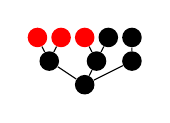
\begin{tikzpicture}[scale=.2]
\node[circle, scale=0.75, fill] (tid0) at (3.75,1.5){};
\node[circle, scale=0.75, fill] (tid1) at (1.5,3){};
\node[circle, scale=0.75, fill, red] (tid4) at (0.75,4.5){};
\node[circle, scale=0.75, fill, red] (tid5) at (2.25,4.5){};
\draw[](tid1) -- (tid4);
\draw[](tid1) -- (tid5);
\node[circle, scale=0.75, fill] (tid2) at (4.5,3){};
\node[circle, scale=0.75, fill, red] (tid6) at (3.75,4.5){};
\node[circle, scale=0.75, fill] (tid7) at (5.25,4.5){};
\draw[](tid2) -- (tid6);
\draw[](tid2) -- (tid7);
\node[circle, scale=0.75, fill] (tid3) at (6.75,3){};
\node[circle, scale=0.75, fill] (tid8) at (6.75,4.5){};
\draw[](tid3) -- (tid8);
\draw[](tid0) -- (tid1);
\draw[](tid0) -- (tid2);
\draw[](tid0) -- (tid3);
\end{tikzpicture}
\nodepart{two}
\footnotesize{4.87551}
\nodepart{three}
\footnotesize{$67\:33$}
};
\node[draw opacity=0, fill opacity=0, anchor=south west] (dummyL) at (-6, -30){};
\node[draw=black, rectangle split, anchor=south west, rectangle split parts=3] (sn0x8aa7c60) at ([xshift=2cm]sn0x8aaac58.south east){
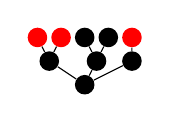
\begin{tikzpicture}[scale=.2]
\node[circle, scale=0.75, fill] (tid0) at (3.75,1.5){};
\node[circle, scale=0.75, fill] (tid1) at (1.5,3){};
\node[circle, scale=0.75, fill, red] (tid4) at (0.75,4.5){};
\node[circle, scale=0.75, fill, red] (tid5) at (2.25,4.5){};
\draw[](tid1) -- (tid4);
\draw[](tid1) -- (tid5);
\node[circle, scale=0.75, fill] (tid2) at (4.5,3){};
\node[circle, scale=0.75, fill] (tid6) at (3.75,4.5){};
\node[circle, scale=0.75, fill] (tid7) at (5.25,4.5){};
\draw[](tid2) -- (tid6);
\draw[](tid2) -- (tid7);
\node[circle, scale=0.75, fill] (tid3) at (6.75,3){};
\node[circle, scale=0.75, fill, red] (tid8) at (6.75,4.5){};
\draw[](tid3) -- (tid8);
\draw[](tid0) -- (tid1);
\draw[](tid0) -- (tid2);
\draw[](tid0) -- (tid3);
\end{tikzpicture}
\nodepart{two}
\footnotesize{4.87243}
\nodepart{three}
\footnotesize{$67\:33$}
};
\node[draw opacity=0, fill opacity=0, anchor=south west] (dummyL) at (-9, -45){};
\node[draw=black, rectangle split, anchor=south west, rectangle split parts=3] (sn0x8aa6428) at ([xshift=2cm]dummyL){
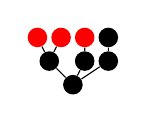
\begin{tikzpicture}[scale=.2]
\node[circle, scale=0.75, fill] (tid0) at (3,1.5){};
\node[circle, scale=0.75, fill] (tid1) at (1.5,3){};
\node[circle, scale=0.75, fill, red] (tid4) at (0.75,4.5){};
\node[circle, scale=0.75, fill, red] (tid5) at (2.25,4.5){};
\draw[](tid1) -- (tid4);
\draw[](tid1) -- (tid5);
\node[circle, scale=0.75, fill] (tid2) at (3.75,3){};
\node[circle, scale=0.75, fill, red] (tid6) at (3.75,4.5){};
\draw[](tid2) -- (tid6);
\node[circle, scale=0.75, fill] (tid3) at (5.25,3){};
\node[circle, scale=0.75, fill] (tid7) at (5.25,4.5){};
\draw[](tid3) -- (tid7);
\draw[](tid0) -- (tid1);
\draw[](tid0) -- (tid2);
\draw[](tid0) -- (tid3);
\end{tikzpicture}
\nodepart{two}
\footnotesize{4.54321}
\nodepart{three}
\footnotesize{$67\:33$}
};
\node[draw opacity=0, fill opacity=0, anchor=south west] (dummyL) at (-9, -45){};
\node[draw=black, rectangle split, anchor=south west, rectangle split parts=3] (sn0x8aa6140) at ([xshift=2cm]sn0x8aa6428.south east){
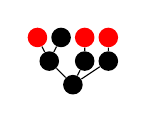
\begin{tikzpicture}[scale=.2]
\node[circle, scale=0.75, fill] (tid0) at (3,1.5){};
\node[circle, scale=0.75, fill] (tid1) at (1.5,3){};
\node[circle, scale=0.75, fill, red] (tid4) at (0.75,4.5){};
\node[circle, scale=0.75, fill] (tid5) at (2.25,4.5){};
\draw[](tid1) -- (tid4);
\draw[](tid1) -- (tid5);
\node[circle, scale=0.75, fill] (tid2) at (3.75,3){};
\node[circle, scale=0.75, fill, red] (tid6) at (3.75,4.5){};
\draw[](tid2) -- (tid6);
\node[circle, scale=0.75, fill] (tid3) at (5.25,3){};
\node[circle, scale=0.75, fill, red] (tid7) at (5.25,4.5){};
\draw[](tid3) -- (tid7);
\draw[](tid0) -- (tid1);
\draw[](tid0) -- (tid2);
\draw[](tid0) -- (tid3);
\end{tikzpicture}
\nodepart{two}
\footnotesize{4.54012}
\nodepart{three}
\footnotesize{$33\:67$}
};
\node[draw opacity=0, fill opacity=0, anchor=south west] (dummyL) at (-9, -45){};
\node[draw=black, rectangle split, anchor=south west, rectangle split parts=3] (sn0x8aabe60) at ([xshift=2cm]sn0x8aa6140.south east){
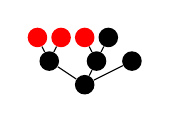
\begin{tikzpicture}[scale=.2]
\node[circle, scale=0.75, fill] (tid0) at (3.75,1.5){};
\node[circle, scale=0.75, fill] (tid1) at (1.5,3){};
\node[circle, scale=0.75, fill, red] (tid4) at (0.75,4.5){};
\node[circle, scale=0.75, fill, red] (tid5) at (2.25,4.5){};
\draw[](tid1) -- (tid4);
\draw[](tid1) -- (tid5);
\node[circle, scale=0.75, fill] (tid2) at (4.5,3){};
\node[circle, scale=0.75, fill, red] (tid6) at (3.75,4.5){};
\node[circle, scale=0.75, fill] (tid7) at (5.25,4.5){};
\draw[](tid2) -- (tid6);
\draw[](tid2) -- (tid7);
\node[circle, scale=0.75, fill] (tid3) at (6.75,3){};
\draw[](tid0) -- (tid1);
\draw[](tid0) -- (tid2);
\draw[](tid0) -- (tid3);
\end{tikzpicture}
\nodepart{two}
\footnotesize{4.53704}
\nodepart{three}
\footnotesize{$1$}
};
\node[draw opacity=0, fill opacity=0, anchor=south west] (dummyL) at (-6, -60){};
\node[draw=black, rectangle split, anchor=south west, rectangle split parts=3] (sn0x8aaaa20) at ([xshift=2cm]dummyL){
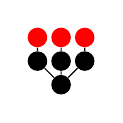
\begin{tikzpicture}[scale=.2]
\node[circle, scale=0.75, fill] (tid0) at (2.25,1.5){};
\node[circle, scale=0.75, fill] (tid1) at (0.75,3){};
\node[circle, scale=0.75, fill, red] (tid4) at (0.75,4.5){};
\draw[](tid1) -- (tid4);
\node[circle, scale=0.75, fill] (tid2) at (2.25,3){};
\node[circle, scale=0.75, fill, red] (tid5) at (2.25,4.5){};
\draw[](tid2) -- (tid5);
\node[circle, scale=0.75, fill] (tid3) at (3.75,3){};
\node[circle, scale=0.75, fill, red] (tid6) at (3.75,4.5){};
\draw[](tid3) -- (tid6);
\draw[](tid0) -- (tid1);
\draw[](tid0) -- (tid2);
\draw[](tid0) -- (tid3);
\end{tikzpicture}
\nodepart{two}
\footnotesize{4.21296}
\nodepart{three}
\footnotesize{$1$}
};
\node[draw opacity=0, fill opacity=0, anchor=south west] (dummyL) at (-6, -60){};
\node[draw=black, rectangle split, anchor=south west, rectangle split parts=3] (sn0x8aaa1e0) at ([xshift=2cm]sn0x8aaaa20.south east){
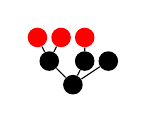
\begin{tikzpicture}[scale=.2]
\node[circle, scale=0.75, fill] (tid0) at (3,1.5){};
\node[circle, scale=0.75, fill] (tid1) at (1.5,3){};
\node[circle, scale=0.75, fill, red] (tid4) at (0.75,4.5){};
\node[circle, scale=0.75, fill, red] (tid5) at (2.25,4.5){};
\draw[](tid1) -- (tid4);
\draw[](tid1) -- (tid5);
\node[circle, scale=0.75, fill] (tid2) at (3.75,3){};
\node[circle, scale=0.75, fill, red] (tid6) at (3.75,4.5){};
\draw[](tid2) -- (tid6);
\node[circle, scale=0.75, fill] (tid3) at (5.25,3){};
\draw[](tid0) -- (tid1);
\draw[](tid0) -- (tid2);
\draw[](tid0) -- (tid3);
\end{tikzpicture}
\nodepart{two}
\footnotesize{4.2037}
\nodepart{three}
\footnotesize{$67\:33$}
};
\node[draw opacity=0, fill opacity=0, anchor=south west] (dummyL) at (-6, -75){};
\node[draw=black, rectangle split, anchor=south west, rectangle split parts=3] (sn0x8aa7da8) at ([xshift=2cm]dummyL){
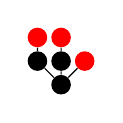
\begin{tikzpicture}[scale=.2]
\node[circle, scale=0.75, fill] (tid0) at (2.25,1.5){};
\node[circle, scale=0.75, fill] (tid1) at (0.75,3){};
\node[circle, scale=0.75, fill, red] (tid4) at (0.75,4.5){};
\draw[](tid1) -- (tid4);
\node[circle, scale=0.75, fill] (tid2) at (2.25,3){};
\node[circle, scale=0.75, fill, red] (tid5) at (2.25,4.5){};
\draw[](tid2) -- (tid5);
\node[circle, scale=0.75, fill, red] (tid3) at (3.75,3){};
\draw[](tid0) -- (tid1);
\draw[](tid0) -- (tid2);
\draw[](tid0) -- (tid3);
\end{tikzpicture}
\nodepart{two}
\footnotesize{3.87963}
\nodepart{three}
\footnotesize{$33\:67$}
};
\node[draw opacity=0, fill opacity=0, anchor=south west] (dummyL) at (-6, -75){};
\node[draw=black, rectangle split, anchor=south west, rectangle split parts=3] (sn0x8aa75f8) at ([xshift=2cm]sn0x8aa7da8.south east){
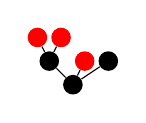
\begin{tikzpicture}[scale=.2]
\node[circle, scale=0.75, fill] (tid0) at (3,1.5){};
\node[circle, scale=0.75, fill] (tid1) at (1.5,3){};
\node[circle, scale=0.75, fill, red] (tid4) at (0.75,4.5){};
\node[circle, scale=0.75, fill, red] (tid5) at (2.25,4.5){};
\draw[](tid1) -- (tid4);
\draw[](tid1) -- (tid5);
\node[circle, scale=0.75, fill, red] (tid2) at (3.75,3){};
\node[circle, scale=0.75, fill] (tid3) at (5.25,3){};
\draw[](tid0) -- (tid1);
\draw[](tid0) -- (tid2);
\draw[](tid0) -- (tid3);
\end{tikzpicture}
\nodepart{two}
\footnotesize{3.85185}
\nodepart{three}
\footnotesize{$67\:33$}
};
\node[draw opacity=0, fill opacity=0, anchor=south west] (dummyL) at (-9, -90){};
\node[draw=black, rectangle split, anchor=south west, rectangle split parts=3] (sn0x8ab1990) at ([xshift=2cm]dummyL){
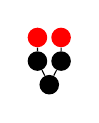
\begin{tikzpicture}[scale=.2]
\node[circle, scale=0.75, fill] (tid0) at (1.5,1.5){};
\node[circle, scale=0.75, fill] (tid1) at (0.75,3){};
\node[circle, scale=0.75, fill, red] (tid3) at (0.75,4.5){};
\draw[](tid1) -- (tid3);
\node[circle, scale=0.75, fill] (tid2) at (2.25,3){};
\node[circle, scale=0.75, fill, red] (tid4) at (2.25,4.5){};
\draw[](tid2) -- (tid4);
\draw[](tid0) -- (tid1);
\draw[](tid0) -- (tid2);
\end{tikzpicture}
\nodepart{two}
\footnotesize{3.75}
\nodepart{three}
\footnotesize{$1$}
};
\node[draw opacity=0, fill opacity=0, anchor=south west] (dummyL) at (-9, -90){};
\node[draw=black, rectangle split, anchor=south west, rectangle split parts=3] (sn0x8aabdc8) at ([xshift=2cm]sn0x8ab1990.south east){
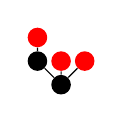
\begin{tikzpicture}[scale=.2]
\node[circle, scale=0.75, fill] (tid0) at (2.25,1.5){};
\node[circle, scale=0.75, fill] (tid1) at (0.75,3){};
\node[circle, scale=0.75, fill, red] (tid4) at (0.75,4.5){};
\draw[](tid1) -- (tid4);
\node[circle, scale=0.75, fill, red] (tid2) at (2.25,3){};
\node[circle, scale=0.75, fill, red] (tid3) at (3.75,3){};
\draw[](tid0) -- (tid1);
\draw[](tid0) -- (tid2);
\draw[](tid0) -- (tid3);
\end{tikzpicture}
\nodepart{two}
\footnotesize{3.44444}
\nodepart{three}
\footnotesize{$67\:33$}
};
\node[draw opacity=0, fill opacity=0, anchor=south west] (dummyL) at (-9, -90){};
\node[draw=black, rectangle split, anchor=south west, rectangle split parts=3] (sn0x8ab1580) at ([xshift=2cm]sn0x8aabdc8.south east){
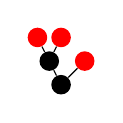
\begin{tikzpicture}[scale=.2]
\node[circle, scale=0.75, fill] (tid0) at (2.25,1.5){};
\node[circle, scale=0.75, fill] (tid1) at (1.5,3){};
\node[circle, scale=0.75, fill, red] (tid3) at (0.75,4.5){};
\node[circle, scale=0.75, fill, red] (tid4) at (2.25,4.5){};
\draw[](tid1) -- (tid3);
\draw[](tid1) -- (tid4);
\node[circle, scale=0.75, fill, red] (tid2) at (3.75,3){};
\draw[](tid0) -- (tid1);
\draw[](tid0) -- (tid2);
\end{tikzpicture}
\nodepart{two}
\footnotesize{3.66667}
\nodepart{three}
\footnotesize{$67\:33$}
};
\node[draw opacity=0, fill opacity=0, anchor=south west] (dummyL) at (-9, -105){};
\node[draw=black, rectangle split, anchor=south west, rectangle split parts=3] (sn0x8aaaab8) at ([xshift=2cm]dummyL){
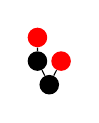
\begin{tikzpicture}[scale=.2]
\node[circle, scale=0.75, fill] (tid0) at (1.5,1.5){};
\node[circle, scale=0.75, fill] (tid1) at (0.75,3){};
\node[circle, scale=0.75, fill, red] (tid3) at (0.75,4.5){};
\draw[](tid1) -- (tid3);
\node[circle, scale=0.75, fill, red] (tid2) at (2.25,3){};
\draw[](tid0) -- (tid1);
\draw[](tid0) -- (tid2);
\end{tikzpicture}
\nodepart{two}
\footnotesize{3.25}
\nodepart{three}
\footnotesize{$50\:50$}
};
\node[draw opacity=0, fill opacity=0, anchor=south west] (dummyL) at (-9, -105){};
\node[draw=black, rectangle split, anchor=south west, rectangle split parts=3] (sn0x8aa7300) at ([xshift=2cm]sn0x8aaaab8.south east){
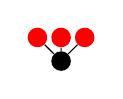
\begin{tikzpicture}[scale=.2]
\node[circle, scale=0.75, fill] (tid0) at (2.25,1.5){};
\node[circle, scale=0.75, fill, red] (tid1) at (0.75,3){};
\node[circle, scale=0.75, fill, red] (tid2) at (2.25,3){};
\node[circle, scale=0.75, fill, red] (tid3) at (3.75,3){};
\draw[](tid0) -- (tid1);
\draw[](tid0) -- (tid2);
\draw[](tid0) -- (tid3);
\end{tikzpicture}
\nodepart{two}
\footnotesize{2.83333}
\nodepart{three}
\footnotesize{$1$}
};
\node[draw opacity=0, fill opacity=0, anchor=south west] (dummyL) at (-9, -105){};
\node[draw=black, rectangle split, anchor=south west, rectangle split parts=3] (sn0x8aad318) at ([xshift=2cm]sn0x8aa7300.south east){
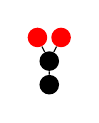
\begin{tikzpicture}[scale=.2]
\node[circle, scale=0.75, fill] (tid0) at (1.5,1.5){};
\node[circle, scale=0.75, fill] (tid1) at (1.5,3){};
\node[circle, scale=0.75, fill, red] (tid2) at (0.75,4.5){};
\node[circle, scale=0.75, fill, red] (tid3) at (2.25,4.5){};
\draw[](tid1) -- (tid2);
\draw[](tid1) -- (tid3);
\draw[](tid0) -- (tid1);
\end{tikzpicture}
\nodepart{two}
\footnotesize{3.5}
\nodepart{three}
\footnotesize{$1$}
};
\node[draw opacity=0, fill opacity=0, anchor=south west] (dummyL) at (-6, -120){};
\node[draw=black, rectangle split, anchor=south west, rectangle split parts=3] (sn0x8ab2230) at ([xshift=2cm]dummyL){
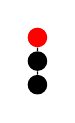
\begin{tikzpicture}[scale=.2]
\node[circle, scale=0.75, fill] (tid0) at (0.75,1.5){};
\node[circle, scale=0.75, fill] (tid1) at (0.75,3){};
\node[circle, scale=0.75, fill, red] (tid2) at (0.75,4.5){};
\draw[](tid1) -- (tid2);
\draw[](tid0) -- (tid1);
\end{tikzpicture}
\nodepart{two}
\footnotesize{3}
\nodepart{three}
\footnotesize{$1$}
};
\node[draw opacity=0, fill opacity=0, anchor=south west] (dummyL) at (-6, -120){};
\node[draw=black, rectangle split, anchor=south west, rectangle split parts=3] (sn0x8aa7130) at ([xshift=2cm]sn0x8ab2230.south east){

\begin{tikzpicture}[scale=.2]
\node[circle, scale=0.75, fill] (tid0) at (1.5,1.5){};
\node[circle, scale=0.75, fill, red] (tid1) at (0.75,3){};
\node[circle, scale=0.75, fill, red] (tid2) at (2.25,3){};
\draw[](tid0) -- (tid1);
\draw[](tid0) -- (tid2);
\end{tikzpicture}
\nodepart{two}
\footnotesize{2.5}
\nodepart{three}
\footnotesize{$1$}
};
\node[draw opacity=0, fill opacity=0, anchor=south west] (dummyL) at (-3, -135){};
\node[draw=black, rectangle split, anchor=south west, rectangle split parts=3] (sn0x8aa7540) at ([xshift=2cm]dummyL){

\begin{tikzpicture}[scale=.2]
\node[circle, scale=0.75, fill] (tid0) at (0.75,1.5){};
\node[circle, scale=0.75, fill, red] (tid1) at (0.75,3){};
\draw[](tid0) -- (tid1);
\end{tikzpicture}
\nodepart{two}
\footnotesize{2}
\nodepart{three}
\footnotesize{$1$}
};
\node[draw opacity=0, fill opacity=0, anchor=south west] (dummyL) at (-3, -150){};
\node[draw=black, rectangle split, anchor=south west, rectangle split parts=3] (sn0x8aa77e0) at ([xshift=2cm]dummyL){

\begin{tikzpicture}[scale=.2]
\node[circle, scale=0.75, fill, red] (tid0) at (0.75,1.5){};
\end{tikzpicture}
\nodepart{two}
\footnotesize{1}
\nodepart{three}
\footnotesize{$$}
};
\draw (sn0x8aa81c0.south) -- (sn0x8aaac58.north);
\draw (sn0x8aa81c0.south) -- (sn0x8aa7c60.north);
\draw (sn0x8aaac58.south) -- (sn0x8aa6428.north);
\draw (sn0x8aaac58.south) -- (sn0x8aa6140.north);
\draw (sn0x8aa7c60.south) -- (sn0x8aa6140.north);
\draw (sn0x8aa7c60.south) -- (sn0x8aabe60.north);
\draw (sn0x8aa6428.south) -- (sn0x8aaaa20.north);
\draw (sn0x8aa6428.south) -- (sn0x8aaa1e0.north);
\draw (sn0x8aa6140.south) -- (sn0x8aaaa20.north);
\draw (sn0x8aa6140.south) -- (sn0x8aaa1e0.north);
\draw (sn0x8aabe60.south) -- (sn0x8aaa1e0.north);
\draw (sn0x8aaaa20.south) -- (sn0x8aa7da8.north);
\draw (sn0x8aaa1e0.south) -- (sn0x8aa7da8.north);
\draw (sn0x8aaa1e0.south) -- (sn0x8aa75f8.north);
\draw (sn0x8aa7da8.south) -- (sn0x8ab1990.north);
\draw (sn0x8aa7da8.south) -- (sn0x8aabdc8.north);
\draw (sn0x8aa75f8.south) -- (sn0x8ab1580.north);
\draw (sn0x8aa75f8.south) -- (sn0x8aabdc8.north);
\draw (sn0x8ab1990.south) -- (sn0x8aaaab8.north);
\draw (sn0x8aabdc8.south) -- (sn0x8aaaab8.north);
\draw (sn0x8aabdc8.south) -- (sn0x8aa7300.north);
\draw (sn0x8ab1580.south) -- (sn0x8aad318.north);
\draw (sn0x8ab1580.south) -- (sn0x8aaaab8.north);
\draw (sn0x8aaaab8.south) -- (sn0x8ab2230.north);
\draw (sn0x8aaaab8.south) -- (sn0x8aa7130.north);
\draw (sn0x8aa7300.south) -- (sn0x8aa7130.north);
\draw (sn0x8aad318.south) -- (sn0x8ab2230.north);
\draw (sn0x8ab2230.south) -- (sn0x8aa7540.north);
\draw (sn0x8aa7130.south) -- (sn0x8aa7540.north);
\draw (sn0x8aa7540.south) -- (sn0x8aa77e0.north);
\end{tikzpicture}

%%% Local Variables:
%%% TeX-master: "thesis/thesis.tex"
%%% End: 
\begin{tikzpicture}[scale=.2, anchor=west]
\node[draw opacity=0, fill opacity=0, anchor=south west] (dummyL) at (-3, -15){};
\node[draw=black, rectangle split, anchor=south west, rectangle split parts=3] (sn0x8aa8220) at ([xshift=2cm]dummyL){
\begin{tikzpicture}[scale=.2]
\node[circle, scale=0.75, fill] (tid0) at (4.5,1.5){};
\node[circle, scale=0.75, fill] (tid1) at (2.25,3){};
\node[circle, scale=0.75, fill, red] (tid4) at (0.75,4.5){};
\node[circle, scale=0.75, fill, red] (tid5) at (2.25,4.5){};
\node[circle, scale=0.75, fill] (tid6) at (3.75,4.5){};
\draw[](tid1) -- (tid4);
\draw[](tid1) -- (tid5);
\draw[](tid1) -- (tid6);
\node[circle, scale=0.75, fill] (tid2) at (6,3){};
\node[circle, scale=0.75, fill, red] (tid7) at (5.25,4.5){};
\node[circle, scale=0.75, fill] (tid8) at (6.75,4.5){};
\draw[](tid2) -- (tid7);
\draw[](tid2) -- (tid8);
\node[circle, scale=0.75, fill] (tid3) at (8.25,3){};
\node[circle, scale=0.75, fill] (tid9) at (8.25,4.5){};
\draw[](tid3) -- (tid9);
\draw[](tid0) -- (tid1);
\draw[](tid0) -- (tid2);
\draw[](tid0) -- (tid3);
\end{tikzpicture}
\nodepart{two}
\footnotesize{5.20782}
\nodepart{three}
\footnotesize{$44\:22\:11\:22$}
};
\node[draw opacity=0, fill opacity=0, anchor=south west] (dummyL) at (-12, -30){};
\node[draw=black, rectangle split, anchor=south west, rectangle split parts=3] (sn0x8aaac58) at ([xshift=2cm]dummyL){
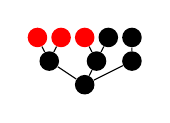
\begin{tikzpicture}[scale=.2]
\node[circle, scale=0.75, fill] (tid0) at (3.75,1.5){};
\node[circle, scale=0.75, fill] (tid1) at (1.5,3){};
\node[circle, scale=0.75, fill, red] (tid4) at (0.75,4.5){};
\node[circle, scale=0.75, fill, red] (tid5) at (2.25,4.5){};
\draw[](tid1) -- (tid4);
\draw[](tid1) -- (tid5);
\node[circle, scale=0.75, fill] (tid2) at (4.5,3){};
\node[circle, scale=0.75, fill, red] (tid6) at (3.75,4.5){};
\node[circle, scale=0.75, fill] (tid7) at (5.25,4.5){};
\draw[](tid2) -- (tid6);
\draw[](tid2) -- (tid7);
\node[circle, scale=0.75, fill] (tid3) at (6.75,3){};
\node[circle, scale=0.75, fill] (tid8) at (6.75,4.5){};
\draw[](tid3) -- (tid8);
\draw[](tid0) -- (tid1);
\draw[](tid0) -- (tid2);
\draw[](tid0) -- (tid3);
\end{tikzpicture}
\nodepart{two}
\footnotesize{4.87551}
\nodepart{three}
\footnotesize{$67\:33$}
};
\node[draw opacity=0, fill opacity=0, anchor=south west] (dummyL) at (-12, -30){};
\node[draw=black, rectangle split, anchor=south west, rectangle split parts=3] (sn0x8aa97b8) at ([xshift=2cm]sn0x8aaac58.south east){
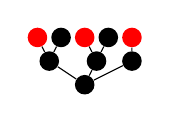
\begin{tikzpicture}[scale=.2]
\node[circle, scale=0.75, fill] (tid0) at (3.75,1.5){};
\node[circle, scale=0.75, fill] (tid1) at (1.5,3){};
\node[circle, scale=0.75, fill, red] (tid4) at (0.75,4.5){};
\node[circle, scale=0.75, fill] (tid5) at (2.25,4.5){};
\draw[](tid1) -- (tid4);
\draw[](tid1) -- (tid5);
\node[circle, scale=0.75, fill] (tid2) at (4.5,3){};
\node[circle, scale=0.75, fill, red] (tid6) at (3.75,4.5){};
\node[circle, scale=0.75, fill] (tid7) at (5.25,4.5){};
\draw[](tid2) -- (tid6);
\draw[](tid2) -- (tid7);
\node[circle, scale=0.75, fill] (tid3) at (6.75,3){};
\node[circle, scale=0.75, fill, red] (tid8) at (6.75,4.5){};
\draw[](tid3) -- (tid8);
\draw[](tid0) -- (tid1);
\draw[](tid0) -- (tid2);
\draw[](tid0) -- (tid3);
\end{tikzpicture}
\nodepart{two}
\footnotesize{4.87346}
\nodepart{three}
\footnotesize{$33\:33\:33$}
};
\node[draw opacity=0, fill opacity=0, anchor=south west] (dummyL) at (-12, -30){};
\node[draw=black, rectangle split, anchor=south west, rectangle split parts=3] (sn0x8aa9030) at ([xshift=2cm]sn0x8aa97b8.south east){
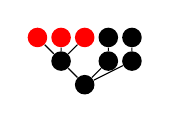
\begin{tikzpicture}[scale=.2]
\node[circle, scale=0.75, fill] (tid0) at (3.75,1.5){};
\node[circle, scale=0.75, fill] (tid1) at (2.25,3){};
\node[circle, scale=0.75, fill, red] (tid4) at (0.75,4.5){};
\node[circle, scale=0.75, fill, red] (tid5) at (2.25,4.5){};
\node[circle, scale=0.75, fill, red] (tid6) at (3.75,4.5){};
\draw[](tid1) -- (tid4);
\draw[](tid1) -- (tid5);
\draw[](tid1) -- (tid6);
\node[circle, scale=0.75, fill] (tid2) at (5.25,3){};
\node[circle, scale=0.75, fill] (tid7) at (5.25,4.5){};
\draw[](tid2) -- (tid7);
\node[circle, scale=0.75, fill] (tid3) at (6.75,3){};
\node[circle, scale=0.75, fill] (tid8) at (6.75,4.5){};
\draw[](tid3) -- (tid8);
\draw[](tid0) -- (tid1);
\draw[](tid0) -- (tid2);
\draw[](tid0) -- (tid3);
\end{tikzpicture}
\nodepart{two}
\footnotesize{4.87654}
\nodepart{three}
\footnotesize{$1$}
};
\node[draw opacity=0, fill opacity=0, anchor=south west] (dummyL) at (-12, -30){};
\node[draw=black, rectangle split, anchor=south west, rectangle split parts=3] (sn0x8ab2a00) at ([xshift=2cm]sn0x8aa9030.south east){
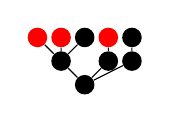
\begin{tikzpicture}[scale=.2]
\node[circle, scale=0.75, fill] (tid0) at (3.75,1.5){};
\node[circle, scale=0.75, fill] (tid1) at (2.25,3){};
\node[circle, scale=0.75, fill, red] (tid4) at (0.75,4.5){};
\node[circle, scale=0.75, fill, red] (tid5) at (2.25,4.5){};
\node[circle, scale=0.75, fill] (tid6) at (3.75,4.5){};
\draw[](tid1) -- (tid4);
\draw[](tid1) -- (tid5);
\draw[](tid1) -- (tid6);
\node[circle, scale=0.75, fill] (tid2) at (5.25,3){};
\node[circle, scale=0.75, fill, red] (tid7) at (5.25,4.5){};
\draw[](tid2) -- (tid7);
\node[circle, scale=0.75, fill] (tid3) at (6.75,3){};
\node[circle, scale=0.75, fill] (tid8) at (6.75,4.5){};
\draw[](tid3) -- (tid8);
\draw[](tid0) -- (tid1);
\draw[](tid0) -- (tid2);
\draw[](tid0) -- (tid3);
\end{tikzpicture}
\nodepart{two}
\footnotesize{4.87243}
\nodepart{three}
\footnotesize{$33\:33\:17\:17$}
};
\node[draw opacity=0, fill opacity=0, anchor=south west] (dummyL) at (-15, -45){};
\node[draw=black, rectangle split, anchor=south west, rectangle split parts=3] (sn0x8aa6428) at ([xshift=2cm]dummyL){
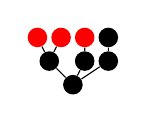
\begin{tikzpicture}[scale=.2]
\node[circle, scale=0.75, fill] (tid0) at (3,1.5){};
\node[circle, scale=0.75, fill] (tid1) at (1.5,3){};
\node[circle, scale=0.75, fill, red] (tid4) at (0.75,4.5){};
\node[circle, scale=0.75, fill, red] (tid5) at (2.25,4.5){};
\draw[](tid1) -- (tid4);
\draw[](tid1) -- (tid5);
\node[circle, scale=0.75, fill] (tid2) at (3.75,3){};
\node[circle, scale=0.75, fill, red] (tid6) at (3.75,4.5){};
\draw[](tid2) -- (tid6);
\node[circle, scale=0.75, fill] (tid3) at (5.25,3){};
\node[circle, scale=0.75, fill] (tid7) at (5.25,4.5){};
\draw[](tid3) -- (tid7);
\draw[](tid0) -- (tid1);
\draw[](tid0) -- (tid2);
\draw[](tid0) -- (tid3);
\end{tikzpicture}
\nodepart{two}
\footnotesize{4.54321}
\nodepart{three}
\footnotesize{$67\:33$}
};
\node[draw opacity=0, fill opacity=0, anchor=south west] (dummyL) at (-15, -45){};
\node[draw=black, rectangle split, anchor=south west, rectangle split parts=3] (sn0x8aa6140) at ([xshift=2cm]sn0x8aa6428.south east){
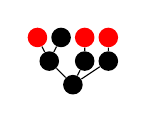
\begin{tikzpicture}[scale=.2]
\node[circle, scale=0.75, fill] (tid0) at (3,1.5){};
\node[circle, scale=0.75, fill] (tid1) at (1.5,3){};
\node[circle, scale=0.75, fill, red] (tid4) at (0.75,4.5){};
\node[circle, scale=0.75, fill] (tid5) at (2.25,4.5){};
\draw[](tid1) -- (tid4);
\draw[](tid1) -- (tid5);
\node[circle, scale=0.75, fill] (tid2) at (3.75,3){};
\node[circle, scale=0.75, fill, red] (tid6) at (3.75,4.5){};
\draw[](tid2) -- (tid6);
\node[circle, scale=0.75, fill] (tid3) at (5.25,3){};
\node[circle, scale=0.75, fill, red] (tid7) at (5.25,4.5){};
\draw[](tid3) -- (tid7);
\draw[](tid0) -- (tid1);
\draw[](tid0) -- (tid2);
\draw[](tid0) -- (tid3);
\end{tikzpicture}
\nodepart{two}
\footnotesize{4.54012}
\nodepart{three}
\footnotesize{$33\:67$}
};
\node[draw opacity=0, fill opacity=0, anchor=south west] (dummyL) at (-15, -45){};
\node[draw=black, rectangle split, anchor=south west, rectangle split parts=3] (sn0x8aabe60) at ([xshift=2cm]sn0x8aa6140.south east){
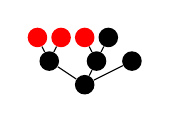
\begin{tikzpicture}[scale=.2]
\node[circle, scale=0.75, fill] (tid0) at (3.75,1.5){};
\node[circle, scale=0.75, fill] (tid1) at (1.5,3){};
\node[circle, scale=0.75, fill, red] (tid4) at (0.75,4.5){};
\node[circle, scale=0.75, fill, red] (tid5) at (2.25,4.5){};
\draw[](tid1) -- (tid4);
\draw[](tid1) -- (tid5);
\node[circle, scale=0.75, fill] (tid2) at (4.5,3){};
\node[circle, scale=0.75, fill, red] (tid6) at (3.75,4.5){};
\node[circle, scale=0.75, fill] (tid7) at (5.25,4.5){};
\draw[](tid2) -- (tid6);
\draw[](tid2) -- (tid7);
\node[circle, scale=0.75, fill] (tid3) at (6.75,3){};
\draw[](tid0) -- (tid1);
\draw[](tid0) -- (tid2);
\draw[](tid0) -- (tid3);
\end{tikzpicture}
\nodepart{two}
\footnotesize{4.53704}
\nodepart{three}
\footnotesize{$1$}
};
\node[draw opacity=0, fill opacity=0, anchor=south west] (dummyL) at (-15, -45){};
\node[draw=black, rectangle split, anchor=south west, rectangle split parts=3] (sn0x8ab3180) at ([xshift=2cm]sn0x8aabe60.south east){
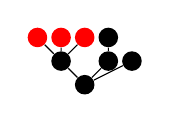
\begin{tikzpicture}[scale=.2]
\node[circle, scale=0.75, fill] (tid0) at (3.75,1.5){};
\node[circle, scale=0.75, fill] (tid1) at (2.25,3){};
\node[circle, scale=0.75, fill, red] (tid4) at (0.75,4.5){};
\node[circle, scale=0.75, fill, red] (tid5) at (2.25,4.5){};
\node[circle, scale=0.75, fill, red] (tid6) at (3.75,4.5){};
\draw[](tid1) -- (tid4);
\draw[](tid1) -- (tid5);
\draw[](tid1) -- (tid6);
\node[circle, scale=0.75, fill] (tid2) at (5.25,3){};
\node[circle, scale=0.75, fill] (tid7) at (5.25,4.5){};
\draw[](tid2) -- (tid7);
\node[circle, scale=0.75, fill] (tid3) at (6.75,3){};
\draw[](tid0) -- (tid1);
\draw[](tid0) -- (tid2);
\draw[](tid0) -- (tid3);
\end{tikzpicture}
\nodepart{two}
\footnotesize{4.53704}
\nodepart{three}
\footnotesize{$1$}
};
\node[draw opacity=0, fill opacity=0, anchor=south west] (dummyL) at (-15, -45){};
\node[draw=black, rectangle split, anchor=south west, rectangle split parts=3] (sn0x8ab3250) at ([xshift=2cm]sn0x8ab3180.south east){
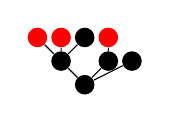
\begin{tikzpicture}[scale=.2]
\node[circle, scale=0.75, fill] (tid0) at (3.75,1.5){};
\node[circle, scale=0.75, fill] (tid1) at (2.25,3){};
\node[circle, scale=0.75, fill, red] (tid4) at (0.75,4.5){};
\node[circle, scale=0.75, fill, red] (tid5) at (2.25,4.5){};
\node[circle, scale=0.75, fill] (tid6) at (3.75,4.5){};
\draw[](tid1) -- (tid4);
\draw[](tid1) -- (tid5);
\draw[](tid1) -- (tid6);
\node[circle, scale=0.75, fill] (tid2) at (5.25,3){};
\node[circle, scale=0.75, fill, red] (tid7) at (5.25,4.5){};
\draw[](tid2) -- (tid7);
\node[circle, scale=0.75, fill] (tid3) at (6.75,3){};
\draw[](tid0) -- (tid1);
\draw[](tid0) -- (tid2);
\draw[](tid0) -- (tid3);
\end{tikzpicture}
\nodepart{two}
\footnotesize{4.53086}
\nodepart{three}
\footnotesize{$67\:33$}
};
\node[draw opacity=0, fill opacity=0, anchor=south west] (dummyL) at (-9, -60){};
\node[draw=black, rectangle split, anchor=south west, rectangle split parts=3] (sn0x8aaaa20) at ([xshift=2cm]dummyL){
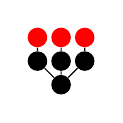
\begin{tikzpicture}[scale=.2]
\node[circle, scale=0.75, fill] (tid0) at (2.25,1.5){};
\node[circle, scale=0.75, fill] (tid1) at (0.75,3){};
\node[circle, scale=0.75, fill, red] (tid4) at (0.75,4.5){};
\draw[](tid1) -- (tid4);
\node[circle, scale=0.75, fill] (tid2) at (2.25,3){};
\node[circle, scale=0.75, fill, red] (tid5) at (2.25,4.5){};
\draw[](tid2) -- (tid5);
\node[circle, scale=0.75, fill] (tid3) at (3.75,3){};
\node[circle, scale=0.75, fill, red] (tid6) at (3.75,4.5){};
\draw[](tid3) -- (tid6);
\draw[](tid0) -- (tid1);
\draw[](tid0) -- (tid2);
\draw[](tid0) -- (tid3);
\end{tikzpicture}
\nodepart{two}
\footnotesize{4.21296}
\nodepart{three}
\footnotesize{$1$}
};
\node[draw opacity=0, fill opacity=0, anchor=south west] (dummyL) at (-9, -60){};
\node[draw=black, rectangle split, anchor=south west, rectangle split parts=3] (sn0x8aaa1e0) at ([xshift=2cm]sn0x8aaaa20.south east){
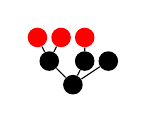
\begin{tikzpicture}[scale=.2]
\node[circle, scale=0.75, fill] (tid0) at (3,1.5){};
\node[circle, scale=0.75, fill] (tid1) at (1.5,3){};
\node[circle, scale=0.75, fill, red] (tid4) at (0.75,4.5){};
\node[circle, scale=0.75, fill, red] (tid5) at (2.25,4.5){};
\draw[](tid1) -- (tid4);
\draw[](tid1) -- (tid5);
\node[circle, scale=0.75, fill] (tid2) at (3.75,3){};
\node[circle, scale=0.75, fill, red] (tid6) at (3.75,4.5){};
\draw[](tid2) -- (tid6);
\node[circle, scale=0.75, fill] (tid3) at (5.25,3){};
\draw[](tid0) -- (tid1);
\draw[](tid0) -- (tid2);
\draw[](tid0) -- (tid3);
\end{tikzpicture}
\nodepart{two}
\footnotesize{4.2037}
\nodepart{three}
\footnotesize{$67\:33$}
};
\node[draw opacity=0, fill opacity=0, anchor=south west] (dummyL) at (-9, -60){};
\node[draw=black, rectangle split, anchor=south west, rectangle split parts=3] (sn0x8ab2630) at ([xshift=2cm]sn0x8aaa1e0.south east){
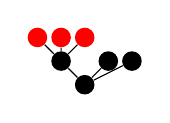
\begin{tikzpicture}[scale=.2]
\node[circle, scale=0.75, fill] (tid0) at (3.75,1.5){};
\node[circle, scale=0.75, fill] (tid1) at (2.25,3){};
\node[circle, scale=0.75, fill, red] (tid4) at (0.75,4.5){};
\node[circle, scale=0.75, fill, red] (tid5) at (2.25,4.5){};
\node[circle, scale=0.75, fill, red] (tid6) at (3.75,4.5){};
\draw[](tid1) -- (tid4);
\draw[](tid1) -- (tid5);
\draw[](tid1) -- (tid6);
\node[circle, scale=0.75, fill] (tid2) at (5.25,3){};
\node[circle, scale=0.75, fill] (tid3) at (6.75,3){};
\draw[](tid0) -- (tid1);
\draw[](tid0) -- (tid2);
\draw[](tid0) -- (tid3);
\end{tikzpicture}
\nodepart{two}
\footnotesize{4.18519}
\nodepart{three}
\footnotesize{$1$}
};
\node[draw opacity=0, fill opacity=0, anchor=south west] (dummyL) at (-6, -75){};
\node[draw=black, rectangle split, anchor=south west, rectangle split parts=3] (sn0x8aa7da8) at ([xshift=2cm]dummyL){
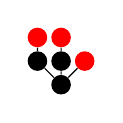
\begin{tikzpicture}[scale=.2]
\node[circle, scale=0.75, fill] (tid0) at (2.25,1.5){};
\node[circle, scale=0.75, fill] (tid1) at (0.75,3){};
\node[circle, scale=0.75, fill, red] (tid4) at (0.75,4.5){};
\draw[](tid1) -- (tid4);
\node[circle, scale=0.75, fill] (tid2) at (2.25,3){};
\node[circle, scale=0.75, fill, red] (tid5) at (2.25,4.5){};
\draw[](tid2) -- (tid5);
\node[circle, scale=0.75, fill, red] (tid3) at (3.75,3){};
\draw[](tid0) -- (tid1);
\draw[](tid0) -- (tid2);
\draw[](tid0) -- (tid3);
\end{tikzpicture}
\nodepart{two}
\footnotesize{3.87963}
\nodepart{three}
\footnotesize{$33\:67$}
};
\node[draw opacity=0, fill opacity=0, anchor=south west] (dummyL) at (-6, -75){};
\node[draw=black, rectangle split, anchor=south west, rectangle split parts=3] (sn0x8aa75f8) at ([xshift=2cm]sn0x8aa7da8.south east){
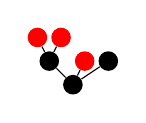
\begin{tikzpicture}[scale=.2]
\node[circle, scale=0.75, fill] (tid0) at (3,1.5){};
\node[circle, scale=0.75, fill] (tid1) at (1.5,3){};
\node[circle, scale=0.75, fill, red] (tid4) at (0.75,4.5){};
\node[circle, scale=0.75, fill, red] (tid5) at (2.25,4.5){};
\draw[](tid1) -- (tid4);
\draw[](tid1) -- (tid5);
\node[circle, scale=0.75, fill, red] (tid2) at (3.75,3){};
\node[circle, scale=0.75, fill] (tid3) at (5.25,3){};
\draw[](tid0) -- (tid1);
\draw[](tid0) -- (tid2);
\draw[](tid0) -- (tid3);
\end{tikzpicture}
\nodepart{two}
\footnotesize{3.85185}
\nodepart{three}
\footnotesize{$67\:33$}
};
\node[draw opacity=0, fill opacity=0, anchor=south west] (dummyL) at (-9, -90){};
\node[draw=black, rectangle split, anchor=south west, rectangle split parts=3] (sn0x8ab1990) at ([xshift=2cm]dummyL){
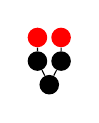
\begin{tikzpicture}[scale=.2]
\node[circle, scale=0.75, fill] (tid0) at (1.5,1.5){};
\node[circle, scale=0.75, fill] (tid1) at (0.75,3){};
\node[circle, scale=0.75, fill, red] (tid3) at (0.75,4.5){};
\draw[](tid1) -- (tid3);
\node[circle, scale=0.75, fill] (tid2) at (2.25,3){};
\node[circle, scale=0.75, fill, red] (tid4) at (2.25,4.5){};
\draw[](tid2) -- (tid4);
\draw[](tid0) -- (tid1);
\draw[](tid0) -- (tid2);
\end{tikzpicture}
\nodepart{two}
\footnotesize{3.75}
\nodepart{three}
\footnotesize{$1$}
};
\node[draw opacity=0, fill opacity=0, anchor=south west] (dummyL) at (-9, -90){};
\node[draw=black, rectangle split, anchor=south west, rectangle split parts=3] (sn0x8aabdc8) at ([xshift=2cm]sn0x8ab1990.south east){
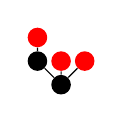
\begin{tikzpicture}[scale=.2]
\node[circle, scale=0.75, fill] (tid0) at (2.25,1.5){};
\node[circle, scale=0.75, fill] (tid1) at (0.75,3){};
\node[circle, scale=0.75, fill, red] (tid4) at (0.75,4.5){};
\draw[](tid1) -- (tid4);
\node[circle, scale=0.75, fill, red] (tid2) at (2.25,3){};
\node[circle, scale=0.75, fill, red] (tid3) at (3.75,3){};
\draw[](tid0) -- (tid1);
\draw[](tid0) -- (tid2);
\draw[](tid0) -- (tid3);
\end{tikzpicture}
\nodepart{two}
\footnotesize{3.44444}
\nodepart{three}
\footnotesize{$67\:33$}
};
\node[draw opacity=0, fill opacity=0, anchor=south west] (dummyL) at (-9, -90){};
\node[draw=black, rectangle split, anchor=south west, rectangle split parts=3] (sn0x8ab1580) at ([xshift=2cm]sn0x8aabdc8.south east){
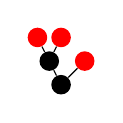
\begin{tikzpicture}[scale=.2]
\node[circle, scale=0.75, fill] (tid0) at (2.25,1.5){};
\node[circle, scale=0.75, fill] (tid1) at (1.5,3){};
\node[circle, scale=0.75, fill, red] (tid3) at (0.75,4.5){};
\node[circle, scale=0.75, fill, red] (tid4) at (2.25,4.5){};
\draw[](tid1) -- (tid3);
\draw[](tid1) -- (tid4);
\node[circle, scale=0.75, fill, red] (tid2) at (3.75,3){};
\draw[](tid0) -- (tid1);
\draw[](tid0) -- (tid2);
\end{tikzpicture}
\nodepart{two}
\footnotesize{3.66667}
\nodepart{three}
\footnotesize{$67\:33$}
};
\node[draw opacity=0, fill opacity=0, anchor=south west] (dummyL) at (-9, -105){};
\node[draw=black, rectangle split, anchor=south west, rectangle split parts=3] (sn0x8aaaab8) at ([xshift=2cm]dummyL){
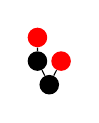
\begin{tikzpicture}[scale=.2]
\node[circle, scale=0.75, fill] (tid0) at (1.5,1.5){};
\node[circle, scale=0.75, fill] (tid1) at (0.75,3){};
\node[circle, scale=0.75, fill, red] (tid3) at (0.75,4.5){};
\draw[](tid1) -- (tid3);
\node[circle, scale=0.75, fill, red] (tid2) at (2.25,3){};
\draw[](tid0) -- (tid1);
\draw[](tid0) -- (tid2);
\end{tikzpicture}
\nodepart{two}
\footnotesize{3.25}
\nodepart{three}
\footnotesize{$50\:50$}
};
\node[draw opacity=0, fill opacity=0, anchor=south west] (dummyL) at (-9, -105){};
\node[draw=black, rectangle split, anchor=south west, rectangle split parts=3] (sn0x8aa7300) at ([xshift=2cm]sn0x8aaaab8.south east){
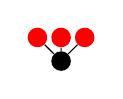
\begin{tikzpicture}[scale=.2]
\node[circle, scale=0.75, fill] (tid0) at (2.25,1.5){};
\node[circle, scale=0.75, fill, red] (tid1) at (0.75,3){};
\node[circle, scale=0.75, fill, red] (tid2) at (2.25,3){};
\node[circle, scale=0.75, fill, red] (tid3) at (3.75,3){};
\draw[](tid0) -- (tid1);
\draw[](tid0) -- (tid2);
\draw[](tid0) -- (tid3);
\end{tikzpicture}
\nodepart{two}
\footnotesize{2.83333}
\nodepart{three}
\footnotesize{$1$}
};
\node[draw opacity=0, fill opacity=0, anchor=south west] (dummyL) at (-9, -105){};
\node[draw=black, rectangle split, anchor=south west, rectangle split parts=3] (sn0x8aad318) at ([xshift=2cm]sn0x8aa7300.south east){
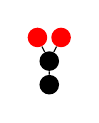
\begin{tikzpicture}[scale=.2]
\node[circle, scale=0.75, fill] (tid0) at (1.5,1.5){};
\node[circle, scale=0.75, fill] (tid1) at (1.5,3){};
\node[circle, scale=0.75, fill, red] (tid2) at (0.75,4.5){};
\node[circle, scale=0.75, fill, red] (tid3) at (2.25,4.5){};
\draw[](tid1) -- (tid2);
\draw[](tid1) -- (tid3);
\draw[](tid0) -- (tid1);
\end{tikzpicture}
\nodepart{two}
\footnotesize{3.5}
\nodepart{three}
\footnotesize{$1$}
};
\node[draw opacity=0, fill opacity=0, anchor=south west] (dummyL) at (-6, -120){};
\node[draw=black, rectangle split, anchor=south west, rectangle split parts=3] (sn0x8ab2230) at ([xshift=2cm]dummyL){
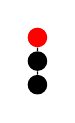
\begin{tikzpicture}[scale=.2]
\node[circle, scale=0.75, fill] (tid0) at (0.75,1.5){};
\node[circle, scale=0.75, fill] (tid1) at (0.75,3){};
\node[circle, scale=0.75, fill, red] (tid2) at (0.75,4.5){};
\draw[](tid1) -- (tid2);
\draw[](tid0) -- (tid1);
\end{tikzpicture}
\nodepart{two}
\footnotesize{3}
\nodepart{three}
\footnotesize{$1$}
};
\node[draw opacity=0, fill opacity=0, anchor=south west] (dummyL) at (-6, -120){};
\node[draw=black, rectangle split, anchor=south west, rectangle split parts=3] (sn0x8aa7130) at ([xshift=2cm]sn0x8ab2230.south east){

\begin{tikzpicture}[scale=.2]
\node[circle, scale=0.75, fill] (tid0) at (1.5,1.5){};
\node[circle, scale=0.75, fill, red] (tid1) at (0.75,3){};
\node[circle, scale=0.75, fill, red] (tid2) at (2.25,3){};
\draw[](tid0) -- (tid1);
\draw[](tid0) -- (tid2);
\end{tikzpicture}
\nodepart{two}
\footnotesize{2.5}
\nodepart{three}
\footnotesize{$1$}
};
\node[draw opacity=0, fill opacity=0, anchor=south west] (dummyL) at (-3, -135){};
\node[draw=black, rectangle split, anchor=south west, rectangle split parts=3] (sn0x8aa7540) at ([xshift=2cm]dummyL){

\begin{tikzpicture}[scale=.2]
\node[circle, scale=0.75, fill] (tid0) at (0.75,1.5){};
\node[circle, scale=0.75, fill, red] (tid1) at (0.75,3){};
\draw[](tid0) -- (tid1);
\end{tikzpicture}
\nodepart{two}
\footnotesize{2}
\nodepart{three}
\footnotesize{$1$}
};
\node[draw opacity=0, fill opacity=0, anchor=south west] (dummyL) at (-3, -150){};
\node[draw=black, rectangle split, anchor=south west, rectangle split parts=3] (sn0x8aa77e0) at ([xshift=2cm]dummyL){

\begin{tikzpicture}[scale=.2]
\node[circle, scale=0.75, fill, red] (tid0) at (0.75,1.5){};
\end{tikzpicture}
\nodepart{two}
\footnotesize{1}
\nodepart{three}
\footnotesize{$$}
};
\draw (sn0x8aa8220.south) -- (sn0x8aaac58.north);
\draw (sn0x8aa8220.south) -- (sn0x8aa97b8.north);
\draw (sn0x8aa8220.south) -- (sn0x8aa9030.north);
\draw (sn0x8aa8220.south) -- (sn0x8ab2a00.north);
\draw (sn0x8aaac58.south) -- (sn0x8aa6428.north);
\draw (sn0x8aaac58.south) -- (sn0x8aa6140.north);
\draw (sn0x8aa97b8.south) -- (sn0x8aa6140.north);
\draw (sn0x8aa97b8.south) -- (sn0x8aa6428.north);
\draw (sn0x8aa97b8.south) -- (sn0x8aabe60.north);
\draw (sn0x8aa9030.south) -- (sn0x8aa6428.north);
\draw (sn0x8ab2a00.south) -- (sn0x8aa6428.north);
\draw (sn0x8ab2a00.south) -- (sn0x8aa6140.north);
\draw (sn0x8ab2a00.south) -- (sn0x8ab3180.north);
\draw (sn0x8ab2a00.south) -- (sn0x8ab3250.north);
\draw (sn0x8aa6428.south) -- (sn0x8aaaa20.north);
\draw (sn0x8aa6428.south) -- (sn0x8aaa1e0.north);
\draw (sn0x8aa6140.south) -- (sn0x8aaaa20.north);
\draw (sn0x8aa6140.south) -- (sn0x8aaa1e0.north);
\draw (sn0x8aabe60.south) -- (sn0x8aaa1e0.north);
\draw (sn0x8ab3180.south) -- (sn0x8aaa1e0.north);
\draw (sn0x8ab3250.south) -- (sn0x8aaa1e0.north);
\draw (sn0x8ab3250.south) -- (sn0x8ab2630.north);
\draw (sn0x8aaaa20.south) -- (sn0x8aa7da8.north);
\draw (sn0x8aaa1e0.south) -- (sn0x8aa7da8.north);
\draw (sn0x8aaa1e0.south) -- (sn0x8aa75f8.north);
\draw (sn0x8ab2630.south) -- (sn0x8aa75f8.north);
\draw (sn0x8aa7da8.south) -- (sn0x8ab1990.north);
\draw (sn0x8aa7da8.south) -- (sn0x8aabdc8.north);
\draw (sn0x8aa75f8.south) -- (sn0x8ab1580.north);
\draw (sn0x8aa75f8.south) -- (sn0x8aabdc8.north);
\draw (sn0x8ab1990.south) -- (sn0x8aaaab8.north);
\draw (sn0x8aabdc8.south) -- (sn0x8aaaab8.north);
\draw (sn0x8aabdc8.south) -- (sn0x8aa7300.north);
\draw (sn0x8ab1580.south) -- (sn0x8aad318.north);
\draw (sn0x8ab1580.south) -- (sn0x8aaaab8.north);
\draw (sn0x8aaaab8.south) -- (sn0x8ab2230.north);
\draw (sn0x8aaaab8.south) -- (sn0x8aa7130.north);
\draw (sn0x8aa7300.south) -- (sn0x8aa7130.north);
\draw (sn0x8aad318.south) -- (sn0x8ab2230.north);
\draw (sn0x8ab2230.south) -- (sn0x8aa7540.north);
\draw (sn0x8aa7130.south) -- (sn0x8aa7540.north);
\draw (sn0x8aa7540.south) -- (sn0x8aa77e0.north);
\end{tikzpicture}

%%% Local Variables:
%%% TeX-master: "thesis/thesis.tex"
%%% End: 
\begin{tikzpicture}[scale=.2, anchor=west]
\node[draw opacity=0, fill opacity=0, anchor=south west] (dummyL) at (-3, -15){};
\node[draw=black, rectangle split, anchor=south west, rectangle split parts=3] (sn0x8aa8280) at ([xshift=2cm]dummyL){
\begin{tikzpicture}[scale=.2]
\node[circle, scale=0.75, fill] (tid0) at (4.5,1.5){};
\node[circle, scale=0.75, fill] (tid1) at (2.25,3){};
\node[circle, scale=0.75, fill, red] (tid4) at (0.75,4.5){};
\node[circle, scale=0.75, fill, red] (tid5) at (2.25,4.5){};
\node[circle, scale=0.75, fill] (tid6) at (3.75,4.5){};
\draw[](tid1) -- (tid4);
\draw[](tid1) -- (tid5);
\draw[](tid1) -- (tid6);
\node[circle, scale=0.75, fill] (tid2) at (6,3){};
\node[circle, scale=0.75, fill] (tid7) at (5.25,4.5){};
\node[circle, scale=0.75, fill] (tid8) at (6.75,4.5){};
\draw[](tid2) -- (tid7);
\draw[](tid2) -- (tid8);
\node[circle, scale=0.75, fill] (tid3) at (8.25,3){};
\node[circle, scale=0.75, fill, red] (tid9) at (8.25,4.5){};
\draw[](tid3) -- (tid9);
\draw[](tid0) -- (tid1);
\draw[](tid0) -- (tid2);
\draw[](tid0) -- (tid3);
\end{tikzpicture}
\nodepart{two}
\footnotesize{5.20531}
\nodepart{three}
\footnotesize{$22\:44\:11\:22$}
};
\node[draw opacity=0, fill opacity=0, anchor=south west] (dummyL) at (-12, -30){};
\node[draw=black, rectangle split, anchor=south west, rectangle split parts=3] (sn0x8aa7c60) at ([xshift=2cm]dummyL){
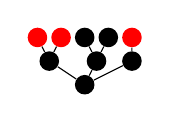
\begin{tikzpicture}[scale=.2]
\node[circle, scale=0.75, fill] (tid0) at (3.75,1.5){};
\node[circle, scale=0.75, fill] (tid1) at (1.5,3){};
\node[circle, scale=0.75, fill, red] (tid4) at (0.75,4.5){};
\node[circle, scale=0.75, fill, red] (tid5) at (2.25,4.5){};
\draw[](tid1) -- (tid4);
\draw[](tid1) -- (tid5);
\node[circle, scale=0.75, fill] (tid2) at (4.5,3){};
\node[circle, scale=0.75, fill] (tid6) at (3.75,4.5){};
\node[circle, scale=0.75, fill] (tid7) at (5.25,4.5){};
\draw[](tid2) -- (tid6);
\draw[](tid2) -- (tid7);
\node[circle, scale=0.75, fill] (tid3) at (6.75,3){};
\node[circle, scale=0.75, fill, red] (tid8) at (6.75,4.5){};
\draw[](tid3) -- (tid8);
\draw[](tid0) -- (tid1);
\draw[](tid0) -- (tid2);
\draw[](tid0) -- (tid3);
\end{tikzpicture}
\nodepart{two}
\footnotesize{4.87243}
\nodepart{three}
\footnotesize{$67\:33$}
};
\node[draw opacity=0, fill opacity=0, anchor=south west] (dummyL) at (-12, -30){};
\node[draw=black, rectangle split, anchor=south west, rectangle split parts=3] (sn0x8aa97b8) at ([xshift=2cm]sn0x8aa7c60.south east){
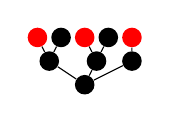
\begin{tikzpicture}[scale=.2]
\node[circle, scale=0.75, fill] (tid0) at (3.75,1.5){};
\node[circle, scale=0.75, fill] (tid1) at (1.5,3){};
\node[circle, scale=0.75, fill, red] (tid4) at (0.75,4.5){};
\node[circle, scale=0.75, fill] (tid5) at (2.25,4.5){};
\draw[](tid1) -- (tid4);
\draw[](tid1) -- (tid5);
\node[circle, scale=0.75, fill] (tid2) at (4.5,3){};
\node[circle, scale=0.75, fill, red] (tid6) at (3.75,4.5){};
\node[circle, scale=0.75, fill] (tid7) at (5.25,4.5){};
\draw[](tid2) -- (tid6);
\draw[](tid2) -- (tid7);
\node[circle, scale=0.75, fill] (tid3) at (6.75,3){};
\node[circle, scale=0.75, fill, red] (tid8) at (6.75,4.5){};
\draw[](tid3) -- (tid8);
\draw[](tid0) -- (tid1);
\draw[](tid0) -- (tid2);
\draw[](tid0) -- (tid3);
\end{tikzpicture}
\nodepart{two}
\footnotesize{4.87346}
\nodepart{three}
\footnotesize{$33\:33\:33$}
};
\node[draw opacity=0, fill opacity=0, anchor=south west] (dummyL) at (-12, -30){};
\node[draw=black, rectangle split, anchor=south west, rectangle split parts=3] (sn0x8ab3e70) at ([xshift=2cm]sn0x8aa97b8.south east){
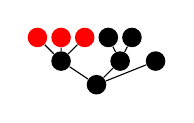
\begin{tikzpicture}[scale=.2]
\node[circle, scale=0.75, fill] (tid0) at (4.5,1.5){};
\node[circle, scale=0.75, fill] (tid1) at (2.25,3){};
\node[circle, scale=0.75, fill, red] (tid4) at (0.75,4.5){};
\node[circle, scale=0.75, fill, red] (tid5) at (2.25,4.5){};
\node[circle, scale=0.75, fill, red] (tid6) at (3.75,4.5){};
\draw[](tid1) -- (tid4);
\draw[](tid1) -- (tid5);
\draw[](tid1) -- (tid6);
\node[circle, scale=0.75, fill] (tid2) at (6,3){};
\node[circle, scale=0.75, fill] (tid7) at (5.25,4.5){};
\node[circle, scale=0.75, fill] (tid8) at (6.75,4.5){};
\draw[](tid2) -- (tid7);
\draw[](tid2) -- (tid8);
\node[circle, scale=0.75, fill] (tid3) at (8.25,3){};
\draw[](tid0) -- (tid1);
\draw[](tid0) -- (tid2);
\draw[](tid0) -- (tid3);
\end{tikzpicture}
\nodepart{two}
\footnotesize{4.87037}
\nodepart{three}
\footnotesize{$1$}
};
\node[draw opacity=0, fill opacity=0, anchor=south west] (dummyL) at (-12, -30){};
\node[draw=black, rectangle split, anchor=south west, rectangle split parts=3] (sn0x8ab3408) at ([xshift=2cm]sn0x8ab3e70.south east){
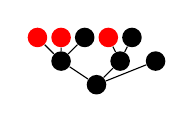
\begin{tikzpicture}[scale=.2]
\node[circle, scale=0.75, fill] (tid0) at (4.5,1.5){};
\node[circle, scale=0.75, fill] (tid1) at (2.25,3){};
\node[circle, scale=0.75, fill, red] (tid4) at (0.75,4.5){};
\node[circle, scale=0.75, fill, red] (tid5) at (2.25,4.5){};
\node[circle, scale=0.75, fill] (tid6) at (3.75,4.5){};
\draw[](tid1) -- (tid4);
\draw[](tid1) -- (tid5);
\draw[](tid1) -- (tid6);
\node[circle, scale=0.75, fill] (tid2) at (6,3){};
\node[circle, scale=0.75, fill, red] (tid7) at (5.25,4.5){};
\node[circle, scale=0.75, fill] (tid8) at (6.75,4.5){};
\draw[](tid2) -- (tid7);
\draw[](tid2) -- (tid8);
\node[circle, scale=0.75, fill] (tid3) at (8.25,3){};
\draw[](tid0) -- (tid1);
\draw[](tid0) -- (tid2);
\draw[](tid0) -- (tid3);
\end{tikzpicture}
\nodepart{two}
\footnotesize{4.86934}
\nodepart{three}
\footnotesize{$67\:17\:17$}
};
\node[draw opacity=0, fill opacity=0, anchor=south west] (dummyL) at (-15, -45){};
\node[draw=black, rectangle split, anchor=south west, rectangle split parts=3] (sn0x8aa6140) at ([xshift=2cm]dummyL){
\begin{tikzpicture}[scale=.2]
\node[circle, scale=0.75, fill] (tid0) at (3,1.5){};
\node[circle, scale=0.75, fill] (tid1) at (1.5,3){};
\node[circle, scale=0.75, fill, red] (tid4) at (0.75,4.5){};
\node[circle, scale=0.75, fill] (tid5) at (2.25,4.5){};
\draw[](tid1) -- (tid4);
\draw[](tid1) -- (tid5);
\node[circle, scale=0.75, fill] (tid2) at (3.75,3){};
\node[circle, scale=0.75, fill, red] (tid6) at (3.75,4.5){};
\draw[](tid2) -- (tid6);
\node[circle, scale=0.75, fill] (tid3) at (5.25,3){};
\node[circle, scale=0.75, fill, red] (tid7) at (5.25,4.5){};
\draw[](tid3) -- (tid7);
\draw[](tid0) -- (tid1);
\draw[](tid0) -- (tid2);
\draw[](tid0) -- (tid3);
\end{tikzpicture}
\nodepart{two}
\footnotesize{4.54012}
\nodepart{three}
\footnotesize{$33\:67$}
};
\node[draw opacity=0, fill opacity=0, anchor=south west] (dummyL) at (-15, -45){};
\node[draw=black, rectangle split, anchor=south west, rectangle split parts=3] (sn0x8aabe60) at ([xshift=2cm]sn0x8aa6140.south east){
\begin{tikzpicture}[scale=.2]
\node[circle, scale=0.75, fill] (tid0) at (3.75,1.5){};
\node[circle, scale=0.75, fill] (tid1) at (1.5,3){};
\node[circle, scale=0.75, fill, red] (tid4) at (0.75,4.5){};
\node[circle, scale=0.75, fill, red] (tid5) at (2.25,4.5){};
\draw[](tid1) -- (tid4);
\draw[](tid1) -- (tid5);
\node[circle, scale=0.75, fill] (tid2) at (4.5,3){};
\node[circle, scale=0.75, fill, red] (tid6) at (3.75,4.5){};
\node[circle, scale=0.75, fill] (tid7) at (5.25,4.5){};
\draw[](tid2) -- (tid6);
\draw[](tid2) -- (tid7);
\node[circle, scale=0.75, fill] (tid3) at (6.75,3){};
\draw[](tid0) -- (tid1);
\draw[](tid0) -- (tid2);
\draw[](tid0) -- (tid3);
\end{tikzpicture}
\nodepart{two}
\footnotesize{4.53704}
\nodepart{three}
\footnotesize{$1$}
};
\node[draw opacity=0, fill opacity=0, anchor=south west] (dummyL) at (-15, -45){};
\node[draw=black, rectangle split, anchor=south west, rectangle split parts=3] (sn0x8aa6428) at ([xshift=2cm]sn0x8aabe60.south east){
\begin{tikzpicture}[scale=.2]
\node[circle, scale=0.75, fill] (tid0) at (3,1.5){};
\node[circle, scale=0.75, fill] (tid1) at (1.5,3){};
\node[circle, scale=0.75, fill, red] (tid4) at (0.75,4.5){};
\node[circle, scale=0.75, fill, red] (tid5) at (2.25,4.5){};
\draw[](tid1) -- (tid4);
\draw[](tid1) -- (tid5);
\node[circle, scale=0.75, fill] (tid2) at (3.75,3){};
\node[circle, scale=0.75, fill, red] (tid6) at (3.75,4.5){};
\draw[](tid2) -- (tid6);
\node[circle, scale=0.75, fill] (tid3) at (5.25,3){};
\node[circle, scale=0.75, fill] (tid7) at (5.25,4.5){};
\draw[](tid3) -- (tid7);
\draw[](tid0) -- (tid1);
\draw[](tid0) -- (tid2);
\draw[](tid0) -- (tid3);
\end{tikzpicture}
\nodepart{two}
\footnotesize{4.54321}
\nodepart{three}
\footnotesize{$67\:33$}
};
\node[draw opacity=0, fill opacity=0, anchor=south west] (dummyL) at (-15, -45){};
\node[draw=black, rectangle split, anchor=south west, rectangle split parts=3] (sn0x8ab3180) at ([xshift=2cm]sn0x8aa6428.south east){
\begin{tikzpicture}[scale=.2]
\node[circle, scale=0.75, fill] (tid0) at (3.75,1.5){};
\node[circle, scale=0.75, fill] (tid1) at (2.25,3){};
\node[circle, scale=0.75, fill, red] (tid4) at (0.75,4.5){};
\node[circle, scale=0.75, fill, red] (tid5) at (2.25,4.5){};
\node[circle, scale=0.75, fill, red] (tid6) at (3.75,4.5){};
\draw[](tid1) -- (tid4);
\draw[](tid1) -- (tid5);
\draw[](tid1) -- (tid6);
\node[circle, scale=0.75, fill] (tid2) at (5.25,3){};
\node[circle, scale=0.75, fill] (tid7) at (5.25,4.5){};
\draw[](tid2) -- (tid7);
\node[circle, scale=0.75, fill] (tid3) at (6.75,3){};
\draw[](tid0) -- (tid1);
\draw[](tid0) -- (tid2);
\draw[](tid0) -- (tid3);
\end{tikzpicture}
\nodepart{two}
\footnotesize{4.53704}
\nodepart{three}
\footnotesize{$1$}
};
\node[draw opacity=0, fill opacity=0, anchor=south west] (dummyL) at (-15, -45){};
\node[draw=black, rectangle split, anchor=south west, rectangle split parts=3] (sn0x8ab3250) at ([xshift=2cm]sn0x8ab3180.south east){
\begin{tikzpicture}[scale=.2]
\node[circle, scale=0.75, fill] (tid0) at (3.75,1.5){};
\node[circle, scale=0.75, fill] (tid1) at (2.25,3){};
\node[circle, scale=0.75, fill, red] (tid4) at (0.75,4.5){};
\node[circle, scale=0.75, fill, red] (tid5) at (2.25,4.5){};
\node[circle, scale=0.75, fill] (tid6) at (3.75,4.5){};
\draw[](tid1) -- (tid4);
\draw[](tid1) -- (tid5);
\draw[](tid1) -- (tid6);
\node[circle, scale=0.75, fill] (tid2) at (5.25,3){};
\node[circle, scale=0.75, fill, red] (tid7) at (5.25,4.5){};
\draw[](tid2) -- (tid7);
\node[circle, scale=0.75, fill] (tid3) at (6.75,3){};
\draw[](tid0) -- (tid1);
\draw[](tid0) -- (tid2);
\draw[](tid0) -- (tid3);
\end{tikzpicture}
\nodepart{two}
\footnotesize{4.53086}
\nodepart{three}
\footnotesize{$67\:33$}
};
\node[draw opacity=0, fill opacity=0, anchor=south west] (dummyL) at (-9, -60){};
\node[draw=black, rectangle split, anchor=south west, rectangle split parts=3] (sn0x8aaaa20) at ([xshift=2cm]dummyL){
\begin{tikzpicture}[scale=.2]
\node[circle, scale=0.75, fill] (tid0) at (2.25,1.5){};
\node[circle, scale=0.75, fill] (tid1) at (0.75,3){};
\node[circle, scale=0.75, fill, red] (tid4) at (0.75,4.5){};
\draw[](tid1) -- (tid4);
\node[circle, scale=0.75, fill] (tid2) at (2.25,3){};
\node[circle, scale=0.75, fill, red] (tid5) at (2.25,4.5){};
\draw[](tid2) -- (tid5);
\node[circle, scale=0.75, fill] (tid3) at (3.75,3){};
\node[circle, scale=0.75, fill, red] (tid6) at (3.75,4.5){};
\draw[](tid3) -- (tid6);
\draw[](tid0) -- (tid1);
\draw[](tid0) -- (tid2);
\draw[](tid0) -- (tid3);
\end{tikzpicture}
\nodepart{two}
\footnotesize{4.21296}
\nodepart{three}
\footnotesize{$1$}
};
\node[draw opacity=0, fill opacity=0, anchor=south west] (dummyL) at (-9, -60){};
\node[draw=black, rectangle split, anchor=south west, rectangle split parts=3] (sn0x8aaa1e0) at ([xshift=2cm]sn0x8aaaa20.south east){
\begin{tikzpicture}[scale=.2]
\node[circle, scale=0.75, fill] (tid0) at (3,1.5){};
\node[circle, scale=0.75, fill] (tid1) at (1.5,3){};
\node[circle, scale=0.75, fill, red] (tid4) at (0.75,4.5){};
\node[circle, scale=0.75, fill, red] (tid5) at (2.25,4.5){};
\draw[](tid1) -- (tid4);
\draw[](tid1) -- (tid5);
\node[circle, scale=0.75, fill] (tid2) at (3.75,3){};
\node[circle, scale=0.75, fill, red] (tid6) at (3.75,4.5){};
\draw[](tid2) -- (tid6);
\node[circle, scale=0.75, fill] (tid3) at (5.25,3){};
\draw[](tid0) -- (tid1);
\draw[](tid0) -- (tid2);
\draw[](tid0) -- (tid3);
\end{tikzpicture}
\nodepart{two}
\footnotesize{4.2037}
\nodepart{three}
\footnotesize{$67\:33$}
};
\node[draw opacity=0, fill opacity=0, anchor=south west] (dummyL) at (-9, -60){};
\node[draw=black, rectangle split, anchor=south west, rectangle split parts=3] (sn0x8ab2630) at ([xshift=2cm]sn0x8aaa1e0.south east){
\begin{tikzpicture}[scale=.2]
\node[circle, scale=0.75, fill] (tid0) at (3.75,1.5){};
\node[circle, scale=0.75, fill] (tid1) at (2.25,3){};
\node[circle, scale=0.75, fill, red] (tid4) at (0.75,4.5){};
\node[circle, scale=0.75, fill, red] (tid5) at (2.25,4.5){};
\node[circle, scale=0.75, fill, red] (tid6) at (3.75,4.5){};
\draw[](tid1) -- (tid4);
\draw[](tid1) -- (tid5);
\draw[](tid1) -- (tid6);
\node[circle, scale=0.75, fill] (tid2) at (5.25,3){};
\node[circle, scale=0.75, fill] (tid3) at (6.75,3){};
\draw[](tid0) -- (tid1);
\draw[](tid0) -- (tid2);
\draw[](tid0) -- (tid3);
\end{tikzpicture}
\nodepart{two}
\footnotesize{4.18519}
\nodepart{three}
\footnotesize{$1$}
};
\node[draw opacity=0, fill opacity=0, anchor=south west] (dummyL) at (-6, -75){};
\node[draw=black, rectangle split, anchor=south west, rectangle split parts=3] (sn0x8aa7da8) at ([xshift=2cm]dummyL){
\begin{tikzpicture}[scale=.2]
\node[circle, scale=0.75, fill] (tid0) at (2.25,1.5){};
\node[circle, scale=0.75, fill] (tid1) at (0.75,3){};
\node[circle, scale=0.75, fill, red] (tid4) at (0.75,4.5){};
\draw[](tid1) -- (tid4);
\node[circle, scale=0.75, fill] (tid2) at (2.25,3){};
\node[circle, scale=0.75, fill, red] (tid5) at (2.25,4.5){};
\draw[](tid2) -- (tid5);
\node[circle, scale=0.75, fill, red] (tid3) at (3.75,3){};
\draw[](tid0) -- (tid1);
\draw[](tid0) -- (tid2);
\draw[](tid0) -- (tid3);
\end{tikzpicture}
\nodepart{two}
\footnotesize{3.87963}
\nodepart{three}
\footnotesize{$33\:67$}
};
\node[draw opacity=0, fill opacity=0, anchor=south west] (dummyL) at (-6, -75){};
\node[draw=black, rectangle split, anchor=south west, rectangle split parts=3] (sn0x8aa75f8) at ([xshift=2cm]sn0x8aa7da8.south east){
\begin{tikzpicture}[scale=.2]
\node[circle, scale=0.75, fill] (tid0) at (3,1.5){};
\node[circle, scale=0.75, fill] (tid1) at (1.5,3){};
\node[circle, scale=0.75, fill, red] (tid4) at (0.75,4.5){};
\node[circle, scale=0.75, fill, red] (tid5) at (2.25,4.5){};
\draw[](tid1) -- (tid4);
\draw[](tid1) -- (tid5);
\node[circle, scale=0.75, fill, red] (tid2) at (3.75,3){};
\node[circle, scale=0.75, fill] (tid3) at (5.25,3){};
\draw[](tid0) -- (tid1);
\draw[](tid0) -- (tid2);
\draw[](tid0) -- (tid3);
\end{tikzpicture}
\nodepart{two}
\footnotesize{3.85185}
\nodepart{three}
\footnotesize{$67\:33$}
};
\node[draw opacity=0, fill opacity=0, anchor=south west] (dummyL) at (-9, -90){};
\node[draw=black, rectangle split, anchor=south west, rectangle split parts=3] (sn0x8ab1990) at ([xshift=2cm]dummyL){
\begin{tikzpicture}[scale=.2]
\node[circle, scale=0.75, fill] (tid0) at (1.5,1.5){};
\node[circle, scale=0.75, fill] (tid1) at (0.75,3){};
\node[circle, scale=0.75, fill, red] (tid3) at (0.75,4.5){};
\draw[](tid1) -- (tid3);
\node[circle, scale=0.75, fill] (tid2) at (2.25,3){};
\node[circle, scale=0.75, fill, red] (tid4) at (2.25,4.5){};
\draw[](tid2) -- (tid4);
\draw[](tid0) -- (tid1);
\draw[](tid0) -- (tid2);
\end{tikzpicture}
\nodepart{two}
\footnotesize{3.75}
\nodepart{three}
\footnotesize{$1$}
};
\node[draw opacity=0, fill opacity=0, anchor=south west] (dummyL) at (-9, -90){};
\node[draw=black, rectangle split, anchor=south west, rectangle split parts=3] (sn0x8aabdc8) at ([xshift=2cm]sn0x8ab1990.south east){
\begin{tikzpicture}[scale=.2]
\node[circle, scale=0.75, fill] (tid0) at (2.25,1.5){};
\node[circle, scale=0.75, fill] (tid1) at (0.75,3){};
\node[circle, scale=0.75, fill, red] (tid4) at (0.75,4.5){};
\draw[](tid1) -- (tid4);
\node[circle, scale=0.75, fill, red] (tid2) at (2.25,3){};
\node[circle, scale=0.75, fill, red] (tid3) at (3.75,3){};
\draw[](tid0) -- (tid1);
\draw[](tid0) -- (tid2);
\draw[](tid0) -- (tid3);
\end{tikzpicture}
\nodepart{two}
\footnotesize{3.44444}
\nodepart{three}
\footnotesize{$67\:33$}
};
\node[draw opacity=0, fill opacity=0, anchor=south west] (dummyL) at (-9, -90){};
\node[draw=black, rectangle split, anchor=south west, rectangle split parts=3] (sn0x8ab1580) at ([xshift=2cm]sn0x8aabdc8.south east){
\begin{tikzpicture}[scale=.2]
\node[circle, scale=0.75, fill] (tid0) at (2.25,1.5){};
\node[circle, scale=0.75, fill] (tid1) at (1.5,3){};
\node[circle, scale=0.75, fill, red] (tid3) at (0.75,4.5){};
\node[circle, scale=0.75, fill, red] (tid4) at (2.25,4.5){};
\draw[](tid1) -- (tid3);
\draw[](tid1) -- (tid4);
\node[circle, scale=0.75, fill, red] (tid2) at (3.75,3){};
\draw[](tid0) -- (tid1);
\draw[](tid0) -- (tid2);
\end{tikzpicture}
\nodepart{two}
\footnotesize{3.66667}
\nodepart{three}
\footnotesize{$67\:33$}
};
\node[draw opacity=0, fill opacity=0, anchor=south west] (dummyL) at (-9, -105){};
\node[draw=black, rectangle split, anchor=south west, rectangle split parts=3] (sn0x8aaaab8) at ([xshift=2cm]dummyL){
\begin{tikzpicture}[scale=.2]
\node[circle, scale=0.75, fill] (tid0) at (1.5,1.5){};
\node[circle, scale=0.75, fill] (tid1) at (0.75,3){};
\node[circle, scale=0.75, fill, red] (tid3) at (0.75,4.5){};
\draw[](tid1) -- (tid3);
\node[circle, scale=0.75, fill, red] (tid2) at (2.25,3){};
\draw[](tid0) -- (tid1);
\draw[](tid0) -- (tid2);
\end{tikzpicture}
\nodepart{two}
\footnotesize{3.25}
\nodepart{three}
\footnotesize{$50\:50$}
};
\node[draw opacity=0, fill opacity=0, anchor=south west] (dummyL) at (-9, -105){};
\node[draw=black, rectangle split, anchor=south west, rectangle split parts=3] (sn0x8aa7300) at ([xshift=2cm]sn0x8aaaab8.south east){
\begin{tikzpicture}[scale=.2]
\node[circle, scale=0.75, fill] (tid0) at (2.25,1.5){};
\node[circle, scale=0.75, fill, red] (tid1) at (0.75,3){};
\node[circle, scale=0.75, fill, red] (tid2) at (2.25,3){};
\node[circle, scale=0.75, fill, red] (tid3) at (3.75,3){};
\draw[](tid0) -- (tid1);
\draw[](tid0) -- (tid2);
\draw[](tid0) -- (tid3);
\end{tikzpicture}
\nodepart{two}
\footnotesize{2.83333}
\nodepart{three}
\footnotesize{$1$}
};
\node[draw opacity=0, fill opacity=0, anchor=south west] (dummyL) at (-9, -105){};
\node[draw=black, rectangle split, anchor=south west, rectangle split parts=3] (sn0x8aad318) at ([xshift=2cm]sn0x8aa7300.south east){
\begin{tikzpicture}[scale=.2]
\node[circle, scale=0.75, fill] (tid0) at (1.5,1.5){};
\node[circle, scale=0.75, fill] (tid1) at (1.5,3){};
\node[circle, scale=0.75, fill, red] (tid2) at (0.75,4.5){};
\node[circle, scale=0.75, fill, red] (tid3) at (2.25,4.5){};
\draw[](tid1) -- (tid2);
\draw[](tid1) -- (tid3);
\draw[](tid0) -- (tid1);
\end{tikzpicture}
\nodepart{two}
\footnotesize{3.5}
\nodepart{three}
\footnotesize{$1$}
};
\node[draw opacity=0, fill opacity=0, anchor=south west] (dummyL) at (-6, -120){};
\node[draw=black, rectangle split, anchor=south west, rectangle split parts=3] (sn0x8ab2230) at ([xshift=2cm]dummyL){
\begin{tikzpicture}[scale=.2]
\node[circle, scale=0.75, fill] (tid0) at (0.75,1.5){};
\node[circle, scale=0.75, fill] (tid1) at (0.75,3){};
\node[circle, scale=0.75, fill, red] (tid2) at (0.75,4.5){};
\draw[](tid1) -- (tid2);
\draw[](tid0) -- (tid1);
\end{tikzpicture}
\nodepart{two}
\footnotesize{3}
\nodepart{three}
\footnotesize{$1$}
};
\node[draw opacity=0, fill opacity=0, anchor=south west] (dummyL) at (-6, -120){};
\node[draw=black, rectangle split, anchor=south west, rectangle split parts=3] (sn0x8aa7130) at ([xshift=2cm]sn0x8ab2230.south east){
\begin{tikzpicture}[scale=.2]
\node[circle, scale=0.75, fill] (tid0) at (1.5,1.5){};
\node[circle, scale=0.75, fill, red] (tid1) at (0.75,3){};
\node[circle, scale=0.75, fill, red] (tid2) at (2.25,3){};
\draw[](tid0) -- (tid1);
\draw[](tid0) -- (tid2);
\end{tikzpicture}
\nodepart{two}
\footnotesize{2.5}
\nodepart{three}
\footnotesize{$1$}
};
\node[draw opacity=0, fill opacity=0, anchor=south west] (dummyL) at (-3, -135){};
\node[draw=black, rectangle split, anchor=south west, rectangle split parts=3] (sn0x8aa7540) at ([xshift=2cm]dummyL){
\begin{tikzpicture}[scale=.2]
\node[circle, scale=0.75, fill] (tid0) at (0.75,1.5){};
\node[circle, scale=0.75, fill, red] (tid1) at (0.75,3){};
\draw[](tid0) -- (tid1);
\end{tikzpicture}
\nodepart{two}
\footnotesize{2}
\nodepart{three}
\footnotesize{$1$}
};
\node[draw opacity=0, fill opacity=0, anchor=south west] (dummyL) at (-3, -150){};
\node[draw=black, rectangle split, anchor=south west, rectangle split parts=3] (sn0x8aa77e0) at ([xshift=2cm]dummyL){
\begin{tikzpicture}[scale=.2]
\node[circle, scale=0.75, fill, red] (tid0) at (0.75,1.5){};
\end{tikzpicture}
\nodepart{two}
\footnotesize{1}
\nodepart{three}
\footnotesize{$$}
};
\draw (sn0x8aa8280.south) -- (sn0x8aa7c60.north);
\draw (sn0x8aa8280.south) -- (sn0x8aa97b8.north);
\draw (sn0x8aa8280.south) -- (sn0x8ab3e70.north);
\draw (sn0x8aa8280.south) -- (sn0x8ab3408.north);
\draw (sn0x8aa7c60.south) -- (sn0x8aa6140.north);
\draw (sn0x8aa7c60.south) -- (sn0x8aabe60.north);
\draw (sn0x8aa97b8.south) -- (sn0x8aa6140.north);
\draw (sn0x8aa97b8.south) -- (sn0x8aa6428.north);
\draw (sn0x8aa97b8.south) -- (sn0x8aabe60.north);
\draw (sn0x8ab3e70.south) -- (sn0x8aabe60.north);
\draw (sn0x8ab3408.south) -- (sn0x8aabe60.north);
\draw (sn0x8ab3408.south) -- (sn0x8ab3180.north);
\draw (sn0x8ab3408.south) -- (sn0x8ab3250.north);
\draw (sn0x8aa6140.south) -- (sn0x8aaaa20.north);
\draw (sn0x8aa6140.south) -- (sn0x8aaa1e0.north);
\draw (sn0x8aabe60.south) -- (sn0x8aaa1e0.north);
\draw (sn0x8aa6428.south) -- (sn0x8aaaa20.north);
\draw (sn0x8aa6428.south) -- (sn0x8aaa1e0.north);
\draw (sn0x8ab3180.south) -- (sn0x8aaa1e0.north);
\draw (sn0x8ab3250.south) -- (sn0x8aaa1e0.north);
\draw (sn0x8ab3250.south) -- (sn0x8ab2630.north);
\draw (sn0x8aaaa20.south) -- (sn0x8aa7da8.north);
\draw (sn0x8aaa1e0.south) -- (sn0x8aa7da8.north);
\draw (sn0x8aaa1e0.south) -- (sn0x8aa75f8.north);
\draw (sn0x8ab2630.south) -- (sn0x8aa75f8.north);
\draw (sn0x8aa7da8.south) -- (sn0x8ab1990.north);
\draw (sn0x8aa7da8.south) -- (sn0x8aabdc8.north);
\draw (sn0x8aa75f8.south) -- (sn0x8ab1580.north);
\draw (sn0x8aa75f8.south) -- (sn0x8aabdc8.north);
\draw (sn0x8ab1990.south) -- (sn0x8aaaab8.north);
\draw (sn0x8aabdc8.south) -- (sn0x8aaaab8.north);
\draw (sn0x8aabdc8.south) -- (sn0x8aa7300.north);
\draw (sn0x8ab1580.south) -- (sn0x8aad318.north);
\draw (sn0x8ab1580.south) -- (sn0x8aaaab8.north);
\draw (sn0x8aaaab8.south) -- (sn0x8ab2230.north);
\draw (sn0x8aaaab8.south) -- (sn0x8aa7130.north);
\draw (sn0x8aa7300.south) -- (sn0x8aa7130.north);
\draw (sn0x8aad318.south) -- (sn0x8ab2230.north);
\draw (sn0x8ab2230.south) -- (sn0x8aa7540.north);
\draw (sn0x8aa7130.south) -- (sn0x8aa7540.north);
\draw (sn0x8aa7540.south) -- (sn0x8aa77e0.north);
\end{tikzpicture}

%%% Local Variables:
%%% TeX-master: "thesis/thesis.tex"
%%% End: 
\begin{tikzpicture}[scale=.2, anchor=west]
\node[draw opacity=0, fill opacity=0, anchor=south west] (dummyL) at (-3, -15){};
\node[draw=black, rectangle split, anchor=south west, rectangle split parts=3] (sn0x8aa82e0) at ([xshift=2cm]dummyL){
\begin{tikzpicture}[scale=.2]
\node[circle, scale=0.75, fill] (tid0) at (4.5,1.5){};
\node[circle, scale=0.75, fill] (tid1) at (2.25,3){};
\node[circle, scale=0.75, fill, red] (tid4) at (0.75,4.5){};
\node[circle, scale=0.75, fill] (tid5) at (2.25,4.5){};
\node[circle, scale=0.75, fill] (tid6) at (3.75,4.5){};
\draw[](tid1) -- (tid4);
\draw[](tid1) -- (tid5);
\draw[](tid1) -- (tid6);
\node[circle, scale=0.75, fill] (tid2) at (6,3){};
\node[circle, scale=0.75, fill, red] (tid7) at (5.25,4.5){};
\node[circle, scale=0.75, fill] (tid8) at (6.75,4.5){};
\draw[](tid2) -- (tid7);
\draw[](tid2) -- (tid8);
\node[circle, scale=0.75, fill] (tid3) at (8.25,3){};
\node[circle, scale=0.75, fill, red] (tid9) at (8.25,4.5){};
\draw[](tid3) -- (tid9);
\draw[](tid0) -- (tid1);
\draw[](tid0) -- (tid2);
\draw[](tid0) -- (tid3);
\end{tikzpicture}
\nodepart{two}
\footnotesize{5.20405}
\nodepart{three}
\footnotesize{$22\:11\:22\:11\:22\:11$}
};
\node[draw opacity=0, fill opacity=0, anchor=south west] (dummyL) at (-18, -30){};
\node[draw=black, rectangle split, anchor=south west, rectangle split parts=3] (sn0x8aa97b8) at ([xshift=2cm]dummyL){
\begin{tikzpicture}[scale=.2]
\node[circle, scale=0.75, fill] (tid0) at (3.75,1.5){};
\node[circle, scale=0.75, fill] (tid1) at (1.5,3){};
\node[circle, scale=0.75, fill, red] (tid4) at (0.75,4.5){};
\node[circle, scale=0.75, fill] (tid5) at (2.25,4.5){};
\draw[](tid1) -- (tid4);
\draw[](tid1) -- (tid5);
\node[circle, scale=0.75, fill] (tid2) at (4.5,3){};
\node[circle, scale=0.75, fill, red] (tid6) at (3.75,4.5){};
\node[circle, scale=0.75, fill] (tid7) at (5.25,4.5){};
\draw[](tid2) -- (tid6);
\draw[](tid2) -- (tid7);
\node[circle, scale=0.75, fill] (tid3) at (6.75,3){};
\node[circle, scale=0.75, fill, red] (tid8) at (6.75,4.5){};
\draw[](tid3) -- (tid8);
\draw[](tid0) -- (tid1);
\draw[](tid0) -- (tid2);
\draw[](tid0) -- (tid3);
\end{tikzpicture}
\nodepart{two}
\footnotesize{4.87346}
\nodepart{three}
\footnotesize{$33\:33\:33$}
};
\node[draw opacity=0, fill opacity=0, anchor=south west] (dummyL) at (-18, -30){};
\node[draw=black, rectangle split, anchor=south west, rectangle split parts=3] (sn0x8aa7c60) at ([xshift=2cm]sn0x8aa97b8.south east){
\begin{tikzpicture}[scale=.2]
\node[circle, scale=0.75, fill] (tid0) at (3.75,1.5){};
\node[circle, scale=0.75, fill] (tid1) at (1.5,3){};
\node[circle, scale=0.75, fill, red] (tid4) at (0.75,4.5){};
\node[circle, scale=0.75, fill, red] (tid5) at (2.25,4.5){};
\draw[](tid1) -- (tid4);
\draw[](tid1) -- (tid5);
\node[circle, scale=0.75, fill] (tid2) at (4.5,3){};
\node[circle, scale=0.75, fill] (tid6) at (3.75,4.5){};
\node[circle, scale=0.75, fill] (tid7) at (5.25,4.5){};
\draw[](tid2) -- (tid6);
\draw[](tid2) -- (tid7);
\node[circle, scale=0.75, fill] (tid3) at (6.75,3){};
\node[circle, scale=0.75, fill, red] (tid8) at (6.75,4.5){};
\draw[](tid3) -- (tid8);
\draw[](tid0) -- (tid1);
\draw[](tid0) -- (tid2);
\draw[](tid0) -- (tid3);
\end{tikzpicture}
\nodepart{two}
\footnotesize{4.87243}
\nodepart{three}
\footnotesize{$67\:33$}
};
\node[draw opacity=0, fill opacity=0, anchor=south west] (dummyL) at (-18, -30){};
\node[draw=black, rectangle split, anchor=south west, rectangle split parts=3] (sn0x8ab2a00) at ([xshift=2cm]sn0x8aa7c60.south east){
\begin{tikzpicture}[scale=.2]
\node[circle, scale=0.75, fill] (tid0) at (3.75,1.5){};
\node[circle, scale=0.75, fill] (tid1) at (2.25,3){};
\node[circle, scale=0.75, fill, red] (tid4) at (0.75,4.5){};
\node[circle, scale=0.75, fill, red] (tid5) at (2.25,4.5){};
\node[circle, scale=0.75, fill] (tid6) at (3.75,4.5){};
\draw[](tid1) -- (tid4);
\draw[](tid1) -- (tid5);
\draw[](tid1) -- (tid6);
\node[circle, scale=0.75, fill] (tid2) at (5.25,3){};
\node[circle, scale=0.75, fill, red] (tid7) at (5.25,4.5){};
\draw[](tid2) -- (tid7);
\node[circle, scale=0.75, fill] (tid3) at (6.75,3){};
\node[circle, scale=0.75, fill] (tid8) at (6.75,4.5){};
\draw[](tid3) -- (tid8);
\draw[](tid0) -- (tid1);
\draw[](tid0) -- (tid2);
\draw[](tid0) -- (tid3);
\end{tikzpicture}
\nodepart{two}
\footnotesize{4.87243}
\nodepart{three}
\footnotesize{$33\:33\:17\:17$}
};
\node[draw opacity=0, fill opacity=0, anchor=south west] (dummyL) at (-18, -30){};
\node[draw=black, rectangle split, anchor=south west, rectangle split parts=3] (sn0x8ab3b48) at ([xshift=2cm]sn0x8ab2a00.south east){
\begin{tikzpicture}[scale=.2]
\node[circle, scale=0.75, fill] (tid0) at (3.75,1.5){};
\node[circle, scale=0.75, fill] (tid1) at (2.25,3){};
\node[circle, scale=0.75, fill, red] (tid4) at (0.75,4.5){};
\node[circle, scale=0.75, fill] (tid5) at (2.25,4.5){};
\node[circle, scale=0.75, fill] (tid6) at (3.75,4.5){};
\draw[](tid1) -- (tid4);
\draw[](tid1) -- (tid5);
\draw[](tid1) -- (tid6);
\node[circle, scale=0.75, fill] (tid2) at (5.25,3){};
\node[circle, scale=0.75, fill, red] (tid7) at (5.25,4.5){};
\draw[](tid2) -- (tid7);
\node[circle, scale=0.75, fill] (tid3) at (6.75,3){};
\node[circle, scale=0.75, fill, red] (tid8) at (6.75,4.5){};
\draw[](tid3) -- (tid8);
\draw[](tid0) -- (tid1);
\draw[](tid0) -- (tid2);
\draw[](tid0) -- (tid3);
\end{tikzpicture}
\nodepart{two}
\footnotesize{4.86728}
\nodepart{three}
\footnotesize{$33\:67$}
};
\node[draw opacity=0, fill opacity=0, anchor=south west] (dummyL) at (-18, -30){};
\node[draw=black, rectangle split, anchor=south west, rectangle split parts=3] (sn0x8ab3408) at ([xshift=2cm]sn0x8ab3b48.south east){
\begin{tikzpicture}[scale=.2]
\node[circle, scale=0.75, fill] (tid0) at (4.5,1.5){};
\node[circle, scale=0.75, fill] (tid1) at (2.25,3){};
\node[circle, scale=0.75, fill, red] (tid4) at (0.75,4.5){};
\node[circle, scale=0.75, fill, red] (tid5) at (2.25,4.5){};
\node[circle, scale=0.75, fill] (tid6) at (3.75,4.5){};
\draw[](tid1) -- (tid4);
\draw[](tid1) -- (tid5);
\draw[](tid1) -- (tid6);
\node[circle, scale=0.75, fill] (tid2) at (6,3){};
\node[circle, scale=0.75, fill, red] (tid7) at (5.25,4.5){};
\node[circle, scale=0.75, fill] (tid8) at (6.75,4.5){};
\draw[](tid2) -- (tid7);
\draw[](tid2) -- (tid8);
\node[circle, scale=0.75, fill] (tid3) at (8.25,3){};
\draw[](tid0) -- (tid1);
\draw[](tid0) -- (tid2);
\draw[](tid0) -- (tid3);
\end{tikzpicture}
\nodepart{two}
\footnotesize{4.86934}
\nodepart{three}
\footnotesize{$67\:17\:17$}
};
\node[draw opacity=0, fill opacity=0, anchor=south west] (dummyL) at (-18, -30){};
\node[draw=black, rectangle split, anchor=south west, rectangle split parts=3] (sn0x8ab48e8) at ([xshift=2cm]sn0x8ab3408.south east){
\begin{tikzpicture}[scale=.2]
\node[circle, scale=0.75, fill] (tid0) at (4.5,1.5){};
\node[circle, scale=0.75, fill] (tid1) at (2.25,3){};
\node[circle, scale=0.75, fill, red] (tid4) at (0.75,4.5){};
\node[circle, scale=0.75, fill] (tid5) at (2.25,4.5){};
\node[circle, scale=0.75, fill] (tid6) at (3.75,4.5){};
\draw[](tid1) -- (tid4);
\draw[](tid1) -- (tid5);
\draw[](tid1) -- (tid6);
\node[circle, scale=0.75, fill] (tid2) at (6,3){};
\node[circle, scale=0.75, fill, red] (tid7) at (5.25,4.5){};
\node[circle, scale=0.75, fill, red] (tid8) at (6.75,4.5){};
\draw[](tid2) -- (tid7);
\draw[](tid2) -- (tid8);
\node[circle, scale=0.75, fill] (tid3) at (8.25,3){};
\draw[](tid0) -- (tid1);
\draw[](tid0) -- (tid2);
\draw[](tid0) -- (tid3);
\end{tikzpicture}
\nodepart{two}
\footnotesize{4.86626}
\nodepart{three}
\footnotesize{$33\:67$}
};
\node[draw opacity=0, fill opacity=0, anchor=south west] (dummyL) at (-15, -45){};
\node[draw=black, rectangle split, anchor=south west, rectangle split parts=3] (sn0x8aa6140) at ([xshift=2cm]dummyL){
\begin{tikzpicture}[scale=.2]
\node[circle, scale=0.75, fill] (tid0) at (3,1.5){};
\node[circle, scale=0.75, fill] (tid1) at (1.5,3){};
\node[circle, scale=0.75, fill, red] (tid4) at (0.75,4.5){};
\node[circle, scale=0.75, fill] (tid5) at (2.25,4.5){};
\draw[](tid1) -- (tid4);
\draw[](tid1) -- (tid5);
\node[circle, scale=0.75, fill] (tid2) at (3.75,3){};
\node[circle, scale=0.75, fill, red] (tid6) at (3.75,4.5){};
\draw[](tid2) -- (tid6);
\node[circle, scale=0.75, fill] (tid3) at (5.25,3){};
\node[circle, scale=0.75, fill, red] (tid7) at (5.25,4.5){};
\draw[](tid3) -- (tid7);
\draw[](tid0) -- (tid1);
\draw[](tid0) -- (tid2);
\draw[](tid0) -- (tid3);
\end{tikzpicture}
\nodepart{two}
\footnotesize{4.54012}
\nodepart{three}
\footnotesize{$33\:67$}
};
\node[draw opacity=0, fill opacity=0, anchor=south west] (dummyL) at (-15, -45){};
\node[draw=black, rectangle split, anchor=south west, rectangle split parts=3] (sn0x8aa6428) at ([xshift=2cm]sn0x8aa6140.south east){
\begin{tikzpicture}[scale=.2]
\node[circle, scale=0.75, fill] (tid0) at (3,1.5){};
\node[circle, scale=0.75, fill] (tid1) at (1.5,3){};
\node[circle, scale=0.75, fill, red] (tid4) at (0.75,4.5){};
\node[circle, scale=0.75, fill, red] (tid5) at (2.25,4.5){};
\draw[](tid1) -- (tid4);
\draw[](tid1) -- (tid5);
\node[circle, scale=0.75, fill] (tid2) at (3.75,3){};
\node[circle, scale=0.75, fill, red] (tid6) at (3.75,4.5){};
\draw[](tid2) -- (tid6);
\node[circle, scale=0.75, fill] (tid3) at (5.25,3){};
\node[circle, scale=0.75, fill] (tid7) at (5.25,4.5){};
\draw[](tid3) -- (tid7);
\draw[](tid0) -- (tid1);
\draw[](tid0) -- (tid2);
\draw[](tid0) -- (tid3);
\end{tikzpicture}
\nodepart{two}
\footnotesize{4.54321}
\nodepart{three}
\footnotesize{$67\:33$}
};
\node[draw opacity=0, fill opacity=0, anchor=south west] (dummyL) at (-15, -45){};
\node[draw=black, rectangle split, anchor=south west, rectangle split parts=3] (sn0x8aabe60) at ([xshift=2cm]sn0x8aa6428.south east){
\begin{tikzpicture}[scale=.2]
\node[circle, scale=0.75, fill] (tid0) at (3.75,1.5){};
\node[circle, scale=0.75, fill] (tid1) at (1.5,3){};
\node[circle, scale=0.75, fill, red] (tid4) at (0.75,4.5){};
\node[circle, scale=0.75, fill, red] (tid5) at (2.25,4.5){};
\draw[](tid1) -- (tid4);
\draw[](tid1) -- (tid5);
\node[circle, scale=0.75, fill] (tid2) at (4.5,3){};
\node[circle, scale=0.75, fill, red] (tid6) at (3.75,4.5){};
\node[circle, scale=0.75, fill] (tid7) at (5.25,4.5){};
\draw[](tid2) -- (tid6);
\draw[](tid2) -- (tid7);
\node[circle, scale=0.75, fill] (tid3) at (6.75,3){};
\draw[](tid0) -- (tid1);
\draw[](tid0) -- (tid2);
\draw[](tid0) -- (tid3);
\end{tikzpicture}
\nodepart{two}
\footnotesize{4.53704}
\nodepart{three}
\footnotesize{$1$}
};
\node[draw opacity=0, fill opacity=0, anchor=south west] (dummyL) at (-15, -45){};
\node[draw=black, rectangle split, anchor=south west, rectangle split parts=3] (sn0x8ab3180) at ([xshift=2cm]sn0x8aabe60.south east){
\begin{tikzpicture}[scale=.2]
\node[circle, scale=0.75, fill] (tid0) at (3.75,1.5){};
\node[circle, scale=0.75, fill] (tid1) at (2.25,3){};
\node[circle, scale=0.75, fill, red] (tid4) at (0.75,4.5){};
\node[circle, scale=0.75, fill, red] (tid5) at (2.25,4.5){};
\node[circle, scale=0.75, fill, red] (tid6) at (3.75,4.5){};
\draw[](tid1) -- (tid4);
\draw[](tid1) -- (tid5);
\draw[](tid1) -- (tid6);
\node[circle, scale=0.75, fill] (tid2) at (5.25,3){};
\node[circle, scale=0.75, fill] (tid7) at (5.25,4.5){};
\draw[](tid2) -- (tid7);
\node[circle, scale=0.75, fill] (tid3) at (6.75,3){};
\draw[](tid0) -- (tid1);
\draw[](tid0) -- (tid2);
\draw[](tid0) -- (tid3);
\end{tikzpicture}
\nodepart{two}
\footnotesize{4.53704}
\nodepart{three}
\footnotesize{$1$}
};
\node[draw opacity=0, fill opacity=0, anchor=south west] (dummyL) at (-15, -45){};
\node[draw=black, rectangle split, anchor=south west, rectangle split parts=3] (sn0x8ab3250) at ([xshift=2cm]sn0x8ab3180.south east){
\begin{tikzpicture}[scale=.2]
\node[circle, scale=0.75, fill] (tid0) at (3.75,1.5){};
\node[circle, scale=0.75, fill] (tid1) at (2.25,3){};
\node[circle, scale=0.75, fill, red] (tid4) at (0.75,4.5){};
\node[circle, scale=0.75, fill, red] (tid5) at (2.25,4.5){};
\node[circle, scale=0.75, fill] (tid6) at (3.75,4.5){};
\draw[](tid1) -- (tid4);
\draw[](tid1) -- (tid5);
\draw[](tid1) -- (tid6);
\node[circle, scale=0.75, fill] (tid2) at (5.25,3){};
\node[circle, scale=0.75, fill, red] (tid7) at (5.25,4.5){};
\draw[](tid2) -- (tid7);
\node[circle, scale=0.75, fill] (tid3) at (6.75,3){};
\draw[](tid0) -- (tid1);
\draw[](tid0) -- (tid2);
\draw[](tid0) -- (tid3);
\end{tikzpicture}
\nodepart{two}
\footnotesize{4.53086}
\nodepart{three}
\footnotesize{$67\:33$}
};
\node[draw opacity=0, fill opacity=0, anchor=south west] (dummyL) at (-9, -60){};
\node[draw=black, rectangle split, anchor=south west, rectangle split parts=3] (sn0x8aaaa20) at ([xshift=2cm]dummyL){
\begin{tikzpicture}[scale=.2]
\node[circle, scale=0.75, fill] (tid0) at (2.25,1.5){};
\node[circle, scale=0.75, fill] (tid1) at (0.75,3){};
\node[circle, scale=0.75, fill, red] (tid4) at (0.75,4.5){};
\draw[](tid1) -- (tid4);
\node[circle, scale=0.75, fill] (tid2) at (2.25,3){};
\node[circle, scale=0.75, fill, red] (tid5) at (2.25,4.5){};
\draw[](tid2) -- (tid5);
\node[circle, scale=0.75, fill] (tid3) at (3.75,3){};
\node[circle, scale=0.75, fill, red] (tid6) at (3.75,4.5){};
\draw[](tid3) -- (tid6);
\draw[](tid0) -- (tid1);
\draw[](tid0) -- (tid2);
\draw[](tid0) -- (tid3);
\end{tikzpicture}
\nodepart{two}
\footnotesize{4.21296}
\nodepart{three}
\footnotesize{$1$}
};
\node[draw opacity=0, fill opacity=0, anchor=south west] (dummyL) at (-9, -60){};
\node[draw=black, rectangle split, anchor=south west, rectangle split parts=3] (sn0x8aaa1e0) at ([xshift=2cm]sn0x8aaaa20.south east){
\begin{tikzpicture}[scale=.2]
\node[circle, scale=0.75, fill] (tid0) at (3,1.5){};
\node[circle, scale=0.75, fill] (tid1) at (1.5,3){};
\node[circle, scale=0.75, fill, red] (tid4) at (0.75,4.5){};
\node[circle, scale=0.75, fill, red] (tid5) at (2.25,4.5){};
\draw[](tid1) -- (tid4);
\draw[](tid1) -- (tid5);
\node[circle, scale=0.75, fill] (tid2) at (3.75,3){};
\node[circle, scale=0.75, fill, red] (tid6) at (3.75,4.5){};
\draw[](tid2) -- (tid6);
\node[circle, scale=0.75, fill] (tid3) at (5.25,3){};
\draw[](tid0) -- (tid1);
\draw[](tid0) -- (tid2);
\draw[](tid0) -- (tid3);
\end{tikzpicture}
\nodepart{two}
\footnotesize{4.2037}
\nodepart{three}
\footnotesize{$67\:33$}
};
\node[draw opacity=0, fill opacity=0, anchor=south west] (dummyL) at (-9, -60){};
\node[draw=black, rectangle split, anchor=south west, rectangle split parts=3] (sn0x8ab2630) at ([xshift=2cm]sn0x8aaa1e0.south east){
\begin{tikzpicture}[scale=.2]
\node[circle, scale=0.75, fill] (tid0) at (3.75,1.5){};
\node[circle, scale=0.75, fill] (tid1) at (2.25,3){};
\node[circle, scale=0.75, fill, red] (tid4) at (0.75,4.5){};
\node[circle, scale=0.75, fill, red] (tid5) at (2.25,4.5){};
\node[circle, scale=0.75, fill, red] (tid6) at (3.75,4.5){};
\draw[](tid1) -- (tid4);
\draw[](tid1) -- (tid5);
\draw[](tid1) -- (tid6);
\node[circle, scale=0.75, fill] (tid2) at (5.25,3){};
\node[circle, scale=0.75, fill] (tid3) at (6.75,3){};
\draw[](tid0) -- (tid1);
\draw[](tid0) -- (tid2);
\draw[](tid0) -- (tid3);
\end{tikzpicture}
\nodepart{two}
\footnotesize{4.18519}
\nodepart{three}
\footnotesize{$1$}
};
\node[draw opacity=0, fill opacity=0, anchor=south west] (dummyL) at (-6, -75){};
\node[draw=black, rectangle split, anchor=south west, rectangle split parts=3] (sn0x8aa7da8) at ([xshift=2cm]dummyL){
\begin{tikzpicture}[scale=.2]
\node[circle, scale=0.75, fill] (tid0) at (2.25,1.5){};
\node[circle, scale=0.75, fill] (tid1) at (0.75,3){};
\node[circle, scale=0.75, fill, red] (tid4) at (0.75,4.5){};
\draw[](tid1) -- (tid4);
\node[circle, scale=0.75, fill] (tid2) at (2.25,3){};
\node[circle, scale=0.75, fill, red] (tid5) at (2.25,4.5){};
\draw[](tid2) -- (tid5);
\node[circle, scale=0.75, fill, red] (tid3) at (3.75,3){};
\draw[](tid0) -- (tid1);
\draw[](tid0) -- (tid2);
\draw[](tid0) -- (tid3);
\end{tikzpicture}
\nodepart{two}
\footnotesize{3.87963}
\nodepart{three}
\footnotesize{$33\:67$}
};
\node[draw opacity=0, fill opacity=0, anchor=south west] (dummyL) at (-6, -75){};
\node[draw=black, rectangle split, anchor=south west, rectangle split parts=3] (sn0x8aa75f8) at ([xshift=2cm]sn0x8aa7da8.south east){
\begin{tikzpicture}[scale=.2]
\node[circle, scale=0.75, fill] (tid0) at (3,1.5){};
\node[circle, scale=0.75, fill] (tid1) at (1.5,3){};
\node[circle, scale=0.75, fill, red] (tid4) at (0.75,4.5){};
\node[circle, scale=0.75, fill, red] (tid5) at (2.25,4.5){};
\draw[](tid1) -- (tid4);
\draw[](tid1) -- (tid5);
\node[circle, scale=0.75, fill, red] (tid2) at (3.75,3){};
\node[circle, scale=0.75, fill] (tid3) at (5.25,3){};
\draw[](tid0) -- (tid1);
\draw[](tid0) -- (tid2);
\draw[](tid0) -- (tid3);
\end{tikzpicture}
\nodepart{two}
\footnotesize{3.85185}
\nodepart{three}
\footnotesize{$67\:33$}
};
\node[draw opacity=0, fill opacity=0, anchor=south west] (dummyL) at (-9, -90){};
\node[draw=black, rectangle split, anchor=south west, rectangle split parts=3] (sn0x8ab1990) at ([xshift=2cm]dummyL){
\begin{tikzpicture}[scale=.2]
\node[circle, scale=0.75, fill] (tid0) at (1.5,1.5){};
\node[circle, scale=0.75, fill] (tid1) at (0.75,3){};
\node[circle, scale=0.75, fill, red] (tid3) at (0.75,4.5){};
\draw[](tid1) -- (tid3);
\node[circle, scale=0.75, fill] (tid2) at (2.25,3){};
\node[circle, scale=0.75, fill, red] (tid4) at (2.25,4.5){};
\draw[](tid2) -- (tid4);
\draw[](tid0) -- (tid1);
\draw[](tid0) -- (tid2);
\end{tikzpicture}
\nodepart{two}
\footnotesize{3.75}
\nodepart{three}
\footnotesize{$1$}
};
\node[draw opacity=0, fill opacity=0, anchor=south west] (dummyL) at (-9, -90){};
\node[draw=black, rectangle split, anchor=south west, rectangle split parts=3] (sn0x8aabdc8) at ([xshift=2cm]sn0x8ab1990.south east){
\begin{tikzpicture}[scale=.2]
\node[circle, scale=0.75, fill] (tid0) at (2.25,1.5){};
\node[circle, scale=0.75, fill] (tid1) at (0.75,3){};
\node[circle, scale=0.75, fill, red] (tid4) at (0.75,4.5){};
\draw[](tid1) -- (tid4);
\node[circle, scale=0.75, fill, red] (tid2) at (2.25,3){};
\node[circle, scale=0.75, fill, red] (tid3) at (3.75,3){};
\draw[](tid0) -- (tid1);
\draw[](tid0) -- (tid2);
\draw[](tid0) -- (tid3);
\end{tikzpicture}
\nodepart{two}
\footnotesize{3.44444}
\nodepart{three}
\footnotesize{$67\:33$}
};
\node[draw opacity=0, fill opacity=0, anchor=south west] (dummyL) at (-9, -90){};
\node[draw=black, rectangle split, anchor=south west, rectangle split parts=3] (sn0x8ab1580) at ([xshift=2cm]sn0x8aabdc8.south east){
\begin{tikzpicture}[scale=.2]
\node[circle, scale=0.75, fill] (tid0) at (2.25,1.5){};
\node[circle, scale=0.75, fill] (tid1) at (1.5,3){};
\node[circle, scale=0.75, fill, red] (tid3) at (0.75,4.5){};
\node[circle, scale=0.75, fill, red] (tid4) at (2.25,4.5){};
\draw[](tid1) -- (tid3);
\draw[](tid1) -- (tid4);
\node[circle, scale=0.75, fill, red] (tid2) at (3.75,3){};
\draw[](tid0) -- (tid1);
\draw[](tid0) -- (tid2);
\end{tikzpicture}
\nodepart{two}
\footnotesize{3.66667}
\nodepart{three}
\footnotesize{$67\:33$}
};
\node[draw opacity=0, fill opacity=0, anchor=south west] (dummyL) at (-9, -105){};
\node[draw=black, rectangle split, anchor=south west, rectangle split parts=3] (sn0x8aaaab8) at ([xshift=2cm]dummyL){
\begin{tikzpicture}[scale=.2]
\node[circle, scale=0.75, fill] (tid0) at (1.5,1.5){};
\node[circle, scale=0.75, fill] (tid1) at (0.75,3){};
\node[circle, scale=0.75, fill, red] (tid3) at (0.75,4.5){};
\draw[](tid1) -- (tid3);
\node[circle, scale=0.75, fill, red] (tid2) at (2.25,3){};
\draw[](tid0) -- (tid1);
\draw[](tid0) -- (tid2);
\end{tikzpicture}
\nodepart{two}
\footnotesize{3.25}
\nodepart{three}
\footnotesize{$50\:50$}
};
\node[draw opacity=0, fill opacity=0, anchor=south west] (dummyL) at (-9, -105){};
\node[draw=black, rectangle split, anchor=south west, rectangle split parts=3] (sn0x8aa7300) at ([xshift=2cm]sn0x8aaaab8.south east){
\begin{tikzpicture}[scale=.2]
\node[circle, scale=0.75, fill] (tid0) at (2.25,1.5){};
\node[circle, scale=0.75, fill, red] (tid1) at (0.75,3){};
\node[circle, scale=0.75, fill, red] (tid2) at (2.25,3){};
\node[circle, scale=0.75, fill, red] (tid3) at (3.75,3){};
\draw[](tid0) -- (tid1);
\draw[](tid0) -- (tid2);
\draw[](tid0) -- (tid3);
\end{tikzpicture}
\nodepart{two}
\footnotesize{2.83333}
\nodepart{three}
\footnotesize{$1$}
};
\node[draw opacity=0, fill opacity=0, anchor=south west] (dummyL) at (-9, -105){};
\node[draw=black, rectangle split, anchor=south west, rectangle split parts=3] (sn0x8aad318) at ([xshift=2cm]sn0x8aa7300.south east){
\begin{tikzpicture}[scale=.2]
\node[circle, scale=0.75, fill] (tid0) at (1.5,1.5){};
\node[circle, scale=0.75, fill] (tid1) at (1.5,3){};
\node[circle, scale=0.75, fill, red] (tid2) at (0.75,4.5){};
\node[circle, scale=0.75, fill, red] (tid3) at (2.25,4.5){};
\draw[](tid1) -- (tid2);
\draw[](tid1) -- (tid3);
\draw[](tid0) -- (tid1);
\end{tikzpicture}
\nodepart{two}
\footnotesize{3.5}
\nodepart{three}
\footnotesize{$1$}
};
\node[draw opacity=0, fill opacity=0, anchor=south west] (dummyL) at (-6, -120){};
\node[draw=black, rectangle split, anchor=south west, rectangle split parts=3] (sn0x8ab2230) at ([xshift=2cm]dummyL){
\begin{tikzpicture}[scale=.2]
\node[circle, scale=0.75, fill] (tid0) at (0.75,1.5){};
\node[circle, scale=0.75, fill] (tid1) at (0.75,3){};
\node[circle, scale=0.75, fill, red] (tid2) at (0.75,4.5){};
\draw[](tid1) -- (tid2);
\draw[](tid0) -- (tid1);
\end{tikzpicture}
\nodepart{two}
\footnotesize{3}
\nodepart{three}
\footnotesize{$1$}
};
\node[draw opacity=0, fill opacity=0, anchor=south west] (dummyL) at (-6, -120){};
\node[draw=black, rectangle split, anchor=south west, rectangle split parts=3] (sn0x8aa7130) at ([xshift=2cm]sn0x8ab2230.south east){
\begin{tikzpicture}[scale=.2]
\node[circle, scale=0.75, fill] (tid0) at (1.5,1.5){};
\node[circle, scale=0.75, fill, red] (tid1) at (0.75,3){};
\node[circle, scale=0.75, fill, red] (tid2) at (2.25,3){};
\draw[](tid0) -- (tid1);
\draw[](tid0) -- (tid2);
\end{tikzpicture}
\nodepart{two}
\footnotesize{2.5}
\nodepart{three}
\footnotesize{$1$}
};
\node[draw opacity=0, fill opacity=0, anchor=south west] (dummyL) at (-3, -135){};
\node[draw=black, rectangle split, anchor=south west, rectangle split parts=3] (sn0x8aa7540) at ([xshift=2cm]dummyL){
\begin{tikzpicture}[scale=.2]
\node[circle, scale=0.75, fill] (tid0) at (0.75,1.5){};
\node[circle, scale=0.75, fill, red] (tid1) at (0.75,3){};
\draw[](tid0) -- (tid1);
\end{tikzpicture}
\nodepart{two}
\footnotesize{2}
\nodepart{three}
\footnotesize{$1$}
};
\node[draw opacity=0, fill opacity=0, anchor=south west] (dummyL) at (-3, -150){};
\node[draw=black, rectangle split, anchor=south west, rectangle split parts=3] (sn0x8aa77e0) at ([xshift=2cm]dummyL){
\begin{tikzpicture}[scale=.2]
\node[circle, scale=0.75, fill, red] (tid0) at (0.75,1.5){};
\end{tikzpicture}
\nodepart{two}
\footnotesize{1}
\nodepart{three}
\footnotesize{$$}
};
\draw (sn0x8aa82e0.south) -- (sn0x8aa97b8.north);
\draw (sn0x8aa82e0.south) -- (sn0x8aa7c60.north);
\draw (sn0x8aa82e0.south) -- (sn0x8ab2a00.north);
\draw (sn0x8aa82e0.south) -- (sn0x8ab3b48.north);
\draw (sn0x8aa82e0.south) -- (sn0x8ab3408.north);
\draw (sn0x8aa82e0.south) -- (sn0x8ab48e8.north);
\draw (sn0x8aa97b8.south) -- (sn0x8aa6140.north);
\draw (sn0x8aa97b8.south) -- (sn0x8aa6428.north);
\draw (sn0x8aa97b8.south) -- (sn0x8aabe60.north);
\draw (sn0x8aa7c60.south) -- (sn0x8aa6140.north);
\draw (sn0x8aa7c60.south) -- (sn0x8aabe60.north);
\draw (sn0x8ab2a00.south) -- (sn0x8aa6428.north);
\draw (sn0x8ab2a00.south) -- (sn0x8aa6140.north);
\draw (sn0x8ab2a00.south) -- (sn0x8ab3180.north);
\draw (sn0x8ab2a00.south) -- (sn0x8ab3250.north);
\draw (sn0x8ab3b48.south) -- (sn0x8aa6140.north);
\draw (sn0x8ab3b48.south) -- (sn0x8ab3250.north);
\draw (sn0x8ab3408.south) -- (sn0x8aabe60.north);
\draw (sn0x8ab3408.south) -- (sn0x8ab3180.north);
\draw (sn0x8ab3408.south) -- (sn0x8ab3250.north);
\draw (sn0x8ab48e8.south) -- (sn0x8aabe60.north);
\draw (sn0x8ab48e8.south) -- (sn0x8ab3250.north);
\draw (sn0x8aa6140.south) -- (sn0x8aaaa20.north);
\draw (sn0x8aa6140.south) -- (sn0x8aaa1e0.north);
\draw (sn0x8aa6428.south) -- (sn0x8aaaa20.north);
\draw (sn0x8aa6428.south) -- (sn0x8aaa1e0.north);
\draw (sn0x8aabe60.south) -- (sn0x8aaa1e0.north);
\draw (sn0x8ab3180.south) -- (sn0x8aaa1e0.north);
\draw (sn0x8ab3250.south) -- (sn0x8aaa1e0.north);
\draw (sn0x8ab3250.south) -- (sn0x8ab2630.north);
\draw (sn0x8aaaa20.south) -- (sn0x8aa7da8.north);
\draw (sn0x8aaa1e0.south) -- (sn0x8aa7da8.north);
\draw (sn0x8aaa1e0.south) -- (sn0x8aa75f8.north);
\draw (sn0x8ab2630.south) -- (sn0x8aa75f8.north);
\draw (sn0x8aa7da8.south) -- (sn0x8ab1990.north);
\draw (sn0x8aa7da8.south) -- (sn0x8aabdc8.north);
\draw (sn0x8aa75f8.south) -- (sn0x8ab1580.north);
\draw (sn0x8aa75f8.south) -- (sn0x8aabdc8.north);
\draw (sn0x8ab1990.south) -- (sn0x8aaaab8.north);
\draw (sn0x8aabdc8.south) -- (sn0x8aaaab8.north);
\draw (sn0x8aabdc8.south) -- (sn0x8aa7300.north);
\draw (sn0x8ab1580.south) -- (sn0x8aad318.north);
\draw (sn0x8ab1580.south) -- (sn0x8aaaab8.north);
\draw (sn0x8aaaab8.south) -- (sn0x8ab2230.north);
\draw (sn0x8aaaab8.south) -- (sn0x8aa7130.north);
\draw (sn0x8aa7300.south) -- (sn0x8aa7130.north);
\draw (sn0x8aad318.south) -- (sn0x8ab2230.north);
\draw (sn0x8ab2230.south) -- (sn0x8aa7540.north);
\draw (sn0x8aa7130.south) -- (sn0x8aa7540.north);
\draw (sn0x8aa7540.south) -- (sn0x8aa77e0.north);
\end{tikzpicture}

%%% Local Variables:
%%% TeX-master: "thesis/thesis.tex"
%%% End: 
\begin{tikzpicture}[scale=.2, anchor=west]
\node[draw opacity=0, fill opacity=0, anchor=south west] (dummyL) at (-3, -15){};
\node[draw=black, rectangle split, anchor=south west, rectangle split parts=3] (sn0x8aa8340) at ([xshift=2cm]dummyL){
\begin{tikzpicture}[scale=.2]
\node[circle, scale=0.75, fill] (tid0) at (4.5,1.5){};
\node[circle, scale=0.75, fill] (tid1) at (2.25,3){};
\node[circle, scale=0.75, fill] (tid4) at (0.75,4.5){};
\node[circle, scale=0.75, fill] (tid5) at (2.25,4.5){};
\node[circle, scale=0.75, fill] (tid6) at (3.75,4.5){};
\draw[](tid1) -- (tid4);
\draw[](tid1) -- (tid5);
\draw[](tid1) -- (tid6);
\node[circle, scale=0.75, fill] (tid2) at (6,3){};
\node[circle, scale=0.75, fill, red] (tid7) at (5.25,4.5){};
\node[circle, scale=0.75, fill, red] (tid8) at (6.75,4.5){};
\draw[](tid2) -- (tid7);
\draw[](tid2) -- (tid8);
\node[circle, scale=0.75, fill] (tid3) at (8.25,3){};
\node[circle, scale=0.75, fill, red] (tid9) at (8.25,4.5){};
\draw[](tid3) -- (tid9);
\draw[](tid0) -- (tid1);
\draw[](tid0) -- (tid2);
\draw[](tid0) -- (tid3);
\end{tikzpicture}
\nodepart{two}
\footnotesize{5.20028}
\nodepart{three}
\footnotesize{$67\:33$}
};
\node[draw opacity=0, fill opacity=0, anchor=south west] (dummyL) at (-6, -30){};
\node[draw=black, rectangle split, anchor=south west, rectangle split parts=3] (sn0x8ab3b48) at ([xshift=2cm]dummyL){
\begin{tikzpicture}[scale=.2]
\node[circle, scale=0.75, fill] (tid0) at (3.75,1.5){};
\node[circle, scale=0.75, fill] (tid1) at (2.25,3){};
\node[circle, scale=0.75, fill, red] (tid4) at (0.75,4.5){};
\node[circle, scale=0.75, fill] (tid5) at (2.25,4.5){};
\node[circle, scale=0.75, fill] (tid6) at (3.75,4.5){};
\draw[](tid1) -- (tid4);
\draw[](tid1) -- (tid5);
\draw[](tid1) -- (tid6);
\node[circle, scale=0.75, fill] (tid2) at (5.25,3){};
\node[circle, scale=0.75, fill, red] (tid7) at (5.25,4.5){};
\draw[](tid2) -- (tid7);
\node[circle, scale=0.75, fill] (tid3) at (6.75,3){};
\node[circle, scale=0.75, fill, red] (tid8) at (6.75,4.5){};
\draw[](tid3) -- (tid8);
\draw[](tid0) -- (tid1);
\draw[](tid0) -- (tid2);
\draw[](tid0) -- (tid3);
\end{tikzpicture}
\nodepart{two}
\footnotesize{4.86728}
\nodepart{three}
\footnotesize{$33\:67$}
};
\node[draw opacity=0, fill opacity=0, anchor=south west] (dummyL) at (-6, -30){};
\node[draw=black, rectangle split, anchor=south west, rectangle split parts=3] (sn0x8ab48e8) at ([xshift=2cm]sn0x8ab3b48.south east){
\begin{tikzpicture}[scale=.2]
\node[circle, scale=0.75, fill] (tid0) at (4.5,1.5){};
\node[circle, scale=0.75, fill] (tid1) at (2.25,3){};
\node[circle, scale=0.75, fill, red] (tid4) at (0.75,4.5){};
\node[circle, scale=0.75, fill] (tid5) at (2.25,4.5){};
\node[circle, scale=0.75, fill] (tid6) at (3.75,4.5){};
\draw[](tid1) -- (tid4);
\draw[](tid1) -- (tid5);
\draw[](tid1) -- (tid6);
\node[circle, scale=0.75, fill] (tid2) at (6,3){};
\node[circle, scale=0.75, fill, red] (tid7) at (5.25,4.5){};
\node[circle, scale=0.75, fill, red] (tid8) at (6.75,4.5){};
\draw[](tid2) -- (tid7);
\draw[](tid2) -- (tid8);
\node[circle, scale=0.75, fill] (tid3) at (8.25,3){};
\draw[](tid0) -- (tid1);
\draw[](tid0) -- (tid2);
\draw[](tid0) -- (tid3);
\end{tikzpicture}
\nodepart{two}
\footnotesize{4.86626}
\nodepart{three}
\footnotesize{$67\:33$}
};
\node[draw opacity=0, fill opacity=0, anchor=south west] (dummyL) at (-9, -45){};
\node[draw=black, rectangle split, anchor=south west, rectangle split parts=3] (sn0x8aa6140) at ([xshift=2cm]dummyL){
\begin{tikzpicture}[scale=.2]
\node[circle, scale=0.75, fill] (tid0) at (3,1.5){};
\node[circle, scale=0.75, fill] (tid1) at (1.5,3){};
\node[circle, scale=0.75, fill, red] (tid4) at (0.75,4.5){};
\node[circle, scale=0.75, fill] (tid5) at (2.25,4.5){};
\draw[](tid1) -- (tid4);
\draw[](tid1) -- (tid5);
\node[circle, scale=0.75, fill] (tid2) at (3.75,3){};
\node[circle, scale=0.75, fill, red] (tid6) at (3.75,4.5){};
\draw[](tid2) -- (tid6);
\node[circle, scale=0.75, fill] (tid3) at (5.25,3){};
\node[circle, scale=0.75, fill, red] (tid7) at (5.25,4.5){};
\draw[](tid3) -- (tid7);
\draw[](tid0) -- (tid1);
\draw[](tid0) -- (tid2);
\draw[](tid0) -- (tid3);
\end{tikzpicture}
\nodepart{two}
\footnotesize{4.54012}
\nodepart{three}
\footnotesize{$33\:67$}
};
\node[draw opacity=0, fill opacity=0, anchor=south west] (dummyL) at (-9, -45){};
\node[draw=black, rectangle split, anchor=south west, rectangle split parts=3] (sn0x8ab3250) at ([xshift=2cm]sn0x8aa6140.south east){
\begin{tikzpicture}[scale=.2]
\node[circle, scale=0.75, fill] (tid0) at (3.75,1.5){};
\node[circle, scale=0.75, fill] (tid1) at (2.25,3){};
\node[circle, scale=0.75, fill, red] (tid4) at (0.75,4.5){};
\node[circle, scale=0.75, fill, red] (tid5) at (2.25,4.5){};
\node[circle, scale=0.75, fill] (tid6) at (3.75,4.5){};
\draw[](tid1) -- (tid4);
\draw[](tid1) -- (tid5);
\draw[](tid1) -- (tid6);
\node[circle, scale=0.75, fill] (tid2) at (5.25,3){};
\node[circle, scale=0.75, fill, red] (tid7) at (5.25,4.5){};
\draw[](tid2) -- (tid7);
\node[circle, scale=0.75, fill] (tid3) at (6.75,3){};
\draw[](tid0) -- (tid1);
\draw[](tid0) -- (tid2);
\draw[](tid0) -- (tid3);
\end{tikzpicture}
\nodepart{two}
\footnotesize{4.53086}
\nodepart{three}
\footnotesize{$67\:33$}
};
\node[draw opacity=0, fill opacity=0, anchor=south west] (dummyL) at (-9, -45){};
\node[draw=black, rectangle split, anchor=south west, rectangle split parts=3] (sn0x8aabe60) at ([xshift=2cm]sn0x8ab3250.south east){
\begin{tikzpicture}[scale=.2]
\node[circle, scale=0.75, fill] (tid0) at (3.75,1.5){};
\node[circle, scale=0.75, fill] (tid1) at (1.5,3){};
\node[circle, scale=0.75, fill, red] (tid4) at (0.75,4.5){};
\node[circle, scale=0.75, fill, red] (tid5) at (2.25,4.5){};
\draw[](tid1) -- (tid4);
\draw[](tid1) -- (tid5);
\node[circle, scale=0.75, fill] (tid2) at (4.5,3){};
\node[circle, scale=0.75, fill, red] (tid6) at (3.75,4.5){};
\node[circle, scale=0.75, fill] (tid7) at (5.25,4.5){};
\draw[](tid2) -- (tid6);
\draw[](tid2) -- (tid7);
\node[circle, scale=0.75, fill] (tid3) at (6.75,3){};
\draw[](tid0) -- (tid1);
\draw[](tid0) -- (tid2);
\draw[](tid0) -- (tid3);
\end{tikzpicture}
\nodepart{two}
\footnotesize{4.53704}
\nodepart{three}
\footnotesize{$1$}
};
\node[draw opacity=0, fill opacity=0, anchor=south west] (dummyL) at (-9, -60){};
\node[draw=black, rectangle split, anchor=south west, rectangle split parts=3] (sn0x8aaaa20) at ([xshift=2cm]dummyL){
\begin{tikzpicture}[scale=.2]
\node[circle, scale=0.75, fill] (tid0) at (2.25,1.5){};
\node[circle, scale=0.75, fill] (tid1) at (0.75,3){};
\node[circle, scale=0.75, fill, red] (tid4) at (0.75,4.5){};
\draw[](tid1) -- (tid4);
\node[circle, scale=0.75, fill] (tid2) at (2.25,3){};
\node[circle, scale=0.75, fill, red] (tid5) at (2.25,4.5){};
\draw[](tid2) -- (tid5);
\node[circle, scale=0.75, fill] (tid3) at (3.75,3){};
\node[circle, scale=0.75, fill, red] (tid6) at (3.75,4.5){};
\draw[](tid3) -- (tid6);
\draw[](tid0) -- (tid1);
\draw[](tid0) -- (tid2);
\draw[](tid0) -- (tid3);
\end{tikzpicture}
\nodepart{two}
\footnotesize{4.21296}
\nodepart{three}
\footnotesize{$1$}
};
\node[draw opacity=0, fill opacity=0, anchor=south west] (dummyL) at (-9, -60){};
\node[draw=black, rectangle split, anchor=south west, rectangle split parts=3] (sn0x8aaa1e0) at ([xshift=2cm]sn0x8aaaa20.south east){
\begin{tikzpicture}[scale=.2]
\node[circle, scale=0.75, fill] (tid0) at (3,1.5){};
\node[circle, scale=0.75, fill] (tid1) at (1.5,3){};
\node[circle, scale=0.75, fill, red] (tid4) at (0.75,4.5){};
\node[circle, scale=0.75, fill, red] (tid5) at (2.25,4.5){};
\draw[](tid1) -- (tid4);
\draw[](tid1) -- (tid5);
\node[circle, scale=0.75, fill] (tid2) at (3.75,3){};
\node[circle, scale=0.75, fill, red] (tid6) at (3.75,4.5){};
\draw[](tid2) -- (tid6);
\node[circle, scale=0.75, fill] (tid3) at (5.25,3){};
\draw[](tid0) -- (tid1);
\draw[](tid0) -- (tid2);
\draw[](tid0) -- (tid3);
\end{tikzpicture}
\nodepart{two}
\footnotesize{4.2037}
\nodepart{three}
\footnotesize{$67\:33$}
};
\node[draw opacity=0, fill opacity=0, anchor=south west] (dummyL) at (-9, -60){};
\node[draw=black, rectangle split, anchor=south west, rectangle split parts=3] (sn0x8ab2630) at ([xshift=2cm]sn0x8aaa1e0.south east){
\begin{tikzpicture}[scale=.2]
\node[circle, scale=0.75, fill] (tid0) at (3.75,1.5){};
\node[circle, scale=0.75, fill] (tid1) at (2.25,3){};
\node[circle, scale=0.75, fill, red] (tid4) at (0.75,4.5){};
\node[circle, scale=0.75, fill, red] (tid5) at (2.25,4.5){};
\node[circle, scale=0.75, fill, red] (tid6) at (3.75,4.5){};
\draw[](tid1) -- (tid4);
\draw[](tid1) -- (tid5);
\draw[](tid1) -- (tid6);
\node[circle, scale=0.75, fill] (tid2) at (5.25,3){};
\node[circle, scale=0.75, fill] (tid3) at (6.75,3){};
\draw[](tid0) -- (tid1);
\draw[](tid0) -- (tid2);
\draw[](tid0) -- (tid3);
\end{tikzpicture}
\nodepart{two}
\footnotesize{4.18519}
\nodepart{three}
\footnotesize{$1$}
};
\node[draw opacity=0, fill opacity=0, anchor=south west] (dummyL) at (-6, -75){};
\node[draw=black, rectangle split, anchor=south west, rectangle split parts=3] (sn0x8aa7da8) at ([xshift=2cm]dummyL){
\begin{tikzpicture}[scale=.2]
\node[circle, scale=0.75, fill] (tid0) at (2.25,1.5){};
\node[circle, scale=0.75, fill] (tid1) at (0.75,3){};
\node[circle, scale=0.75, fill, red] (tid4) at (0.75,4.5){};
\draw[](tid1) -- (tid4);
\node[circle, scale=0.75, fill] (tid2) at (2.25,3){};
\node[circle, scale=0.75, fill, red] (tid5) at (2.25,4.5){};
\draw[](tid2) -- (tid5);
\node[circle, scale=0.75, fill, red] (tid3) at (3.75,3){};
\draw[](tid0) -- (tid1);
\draw[](tid0) -- (tid2);
\draw[](tid0) -- (tid3);
\end{tikzpicture}
\nodepart{two}
\footnotesize{3.87963}
\nodepart{three}
\footnotesize{$33\:67$}
};
\node[draw opacity=0, fill opacity=0, anchor=south west] (dummyL) at (-6, -75){};
\node[draw=black, rectangle split, anchor=south west, rectangle split parts=3] (sn0x8aa75f8) at ([xshift=2cm]sn0x8aa7da8.south east){
\begin{tikzpicture}[scale=.2]
\node[circle, scale=0.75, fill] (tid0) at (3,1.5){};
\node[circle, scale=0.75, fill] (tid1) at (1.5,3){};
\node[circle, scale=0.75, fill, red] (tid4) at (0.75,4.5){};
\node[circle, scale=0.75, fill, red] (tid5) at (2.25,4.5){};
\draw[](tid1) -- (tid4);
\draw[](tid1) -- (tid5);
\node[circle, scale=0.75, fill, red] (tid2) at (3.75,3){};
\node[circle, scale=0.75, fill] (tid3) at (5.25,3){};
\draw[](tid0) -- (tid1);
\draw[](tid0) -- (tid2);
\draw[](tid0) -- (tid3);
\end{tikzpicture}
\nodepart{two}
\footnotesize{3.85185}
\nodepart{three}
\footnotesize{$67\:33$}
};
\node[draw opacity=0, fill opacity=0, anchor=south west] (dummyL) at (-9, -90){};
\node[draw=black, rectangle split, anchor=south west, rectangle split parts=3] (sn0x8ab1990) at ([xshift=2cm]dummyL){
\begin{tikzpicture}[scale=.2]
\node[circle, scale=0.75, fill] (tid0) at (1.5,1.5){};
\node[circle, scale=0.75, fill] (tid1) at (0.75,3){};
\node[circle, scale=0.75, fill, red] (tid3) at (0.75,4.5){};
\draw[](tid1) -- (tid3);
\node[circle, scale=0.75, fill] (tid2) at (2.25,3){};
\node[circle, scale=0.75, fill, red] (tid4) at (2.25,4.5){};
\draw[](tid2) -- (tid4);
\draw[](tid0) -- (tid1);
\draw[](tid0) -- (tid2);
\end{tikzpicture}
\nodepart{two}
\footnotesize{3.75}
\nodepart{three}
\footnotesize{$1$}
};
\node[draw opacity=0, fill opacity=0, anchor=south west] (dummyL) at (-9, -90){};
\node[draw=black, rectangle split, anchor=south west, rectangle split parts=3] (sn0x8aabdc8) at ([xshift=2cm]sn0x8ab1990.south east){
\begin{tikzpicture}[scale=.2]
\node[circle, scale=0.75, fill] (tid0) at (2.25,1.5){};
\node[circle, scale=0.75, fill] (tid1) at (0.75,3){};
\node[circle, scale=0.75, fill, red] (tid4) at (0.75,4.5){};
\draw[](tid1) -- (tid4);
\node[circle, scale=0.75, fill, red] (tid2) at (2.25,3){};
\node[circle, scale=0.75, fill, red] (tid3) at (3.75,3){};
\draw[](tid0) -- (tid1);
\draw[](tid0) -- (tid2);
\draw[](tid0) -- (tid3);
\end{tikzpicture}
\nodepart{two}
\footnotesize{3.44444}
\nodepart{three}
\footnotesize{$67\:33$}
};
\node[draw opacity=0, fill opacity=0, anchor=south west] (dummyL) at (-9, -90){};
\node[draw=black, rectangle split, anchor=south west, rectangle split parts=3] (sn0x8ab1580) at ([xshift=2cm]sn0x8aabdc8.south east){
\begin{tikzpicture}[scale=.2]
\node[circle, scale=0.75, fill] (tid0) at (2.25,1.5){};
\node[circle, scale=0.75, fill] (tid1) at (1.5,3){};
\node[circle, scale=0.75, fill, red] (tid3) at (0.75,4.5){};
\node[circle, scale=0.75, fill, red] (tid4) at (2.25,4.5){};
\draw[](tid1) -- (tid3);
\draw[](tid1) -- (tid4);
\node[circle, scale=0.75, fill, red] (tid2) at (3.75,3){};
\draw[](tid0) -- (tid1);
\draw[](tid0) -- (tid2);
\end{tikzpicture}
\nodepart{two}
\footnotesize{3.66667}
\nodepart{three}
\footnotesize{$67\:33$}
};
\node[draw opacity=0, fill opacity=0, anchor=south west] (dummyL) at (-9, -105){};
\node[draw=black, rectangle split, anchor=south west, rectangle split parts=3] (sn0x8aaaab8) at ([xshift=2cm]dummyL){
\begin{tikzpicture}[scale=.2]
\node[circle, scale=0.75, fill] (tid0) at (1.5,1.5){};
\node[circle, scale=0.75, fill] (tid1) at (0.75,3){};
\node[circle, scale=0.75, fill, red] (tid3) at (0.75,4.5){};
\draw[](tid1) -- (tid3);
\node[circle, scale=0.75, fill, red] (tid2) at (2.25,3){};
\draw[](tid0) -- (tid1);
\draw[](tid0) -- (tid2);
\end{tikzpicture}
\nodepart{two}
\footnotesize{3.25}
\nodepart{three}
\footnotesize{$50\:50$}
};
\node[draw opacity=0, fill opacity=0, anchor=south west] (dummyL) at (-9, -105){};
\node[draw=black, rectangle split, anchor=south west, rectangle split parts=3] (sn0x8aa7300) at ([xshift=2cm]sn0x8aaaab8.south east){
\begin{tikzpicture}[scale=.2]
\node[circle, scale=0.75, fill] (tid0) at (2.25,1.5){};
\node[circle, scale=0.75, fill, red] (tid1) at (0.75,3){};
\node[circle, scale=0.75, fill, red] (tid2) at (2.25,3){};
\node[circle, scale=0.75, fill, red] (tid3) at (3.75,3){};
\draw[](tid0) -- (tid1);
\draw[](tid0) -- (tid2);
\draw[](tid0) -- (tid3);
\end{tikzpicture}
\nodepart{two}
\footnotesize{2.83333}
\nodepart{three}
\footnotesize{$1$}
};
\node[draw opacity=0, fill opacity=0, anchor=south west] (dummyL) at (-9, -105){};
\node[draw=black, rectangle split, anchor=south west, rectangle split parts=3] (sn0x8aad318) at ([xshift=2cm]sn0x8aa7300.south east){
\begin{tikzpicture}[scale=.2]
\node[circle, scale=0.75, fill] (tid0) at (1.5,1.5){};
\node[circle, scale=0.75, fill] (tid1) at (1.5,3){};
\node[circle, scale=0.75, fill, red] (tid2) at (0.75,4.5){};
\node[circle, scale=0.75, fill, red] (tid3) at (2.25,4.5){};
\draw[](tid1) -- (tid2);
\draw[](tid1) -- (tid3);
\draw[](tid0) -- (tid1);
\end{tikzpicture}
\nodepart{two}
\footnotesize{3.5}
\nodepart{three}
\footnotesize{$1$}
};
\node[draw opacity=0, fill opacity=0, anchor=south west] (dummyL) at (-6, -120){};
\node[draw=black, rectangle split, anchor=south west, rectangle split parts=3] (sn0x8ab2230) at ([xshift=2cm]dummyL){
\begin{tikzpicture}[scale=.2]
\node[circle, scale=0.75, fill] (tid0) at (0.75,1.5){};
\node[circle, scale=0.75, fill] (tid1) at (0.75,3){};
\node[circle, scale=0.75, fill, red] (tid2) at (0.75,4.5){};
\draw[](tid1) -- (tid2);
\draw[](tid0) -- (tid1);
\end{tikzpicture}
\nodepart{two}
\footnotesize{3}
\nodepart{three}
\footnotesize{$1$}
};
\node[draw opacity=0, fill opacity=0, anchor=south west] (dummyL) at (-6, -120){};
\node[draw=black, rectangle split, anchor=south west, rectangle split parts=3] (sn0x8aa7130) at ([xshift=2cm]sn0x8ab2230.south east){
\begin{tikzpicture}[scale=.2]
\node[circle, scale=0.75, fill] (tid0) at (1.5,1.5){};
\node[circle, scale=0.75, fill, red] (tid1) at (0.75,3){};
\node[circle, scale=0.75, fill, red] (tid2) at (2.25,3){};
\draw[](tid0) -- (tid1);
\draw[](tid0) -- (tid2);
\end{tikzpicture}
\nodepart{two}
\footnotesize{2.5}
\nodepart{three}
\footnotesize{$1$}
};
\node[draw opacity=0, fill opacity=0, anchor=south west] (dummyL) at (-3, -135){};
\node[draw=black, rectangle split, anchor=south west, rectangle split parts=3] (sn0x8aa7540) at ([xshift=2cm]dummyL){
\begin{tikzpicture}[scale=.2]
\node[circle, scale=0.75, fill] (tid0) at (0.75,1.5){};
\node[circle, scale=0.75, fill, red] (tid1) at (0.75,3){};
\draw[](tid0) -- (tid1);
\end{tikzpicture}
\nodepart{two}
\footnotesize{2}
\nodepart{three}
\footnotesize{$1$}
};
\node[draw opacity=0, fill opacity=0, anchor=south west] (dummyL) at (-3, -150){};
\node[draw=black, rectangle split, anchor=south west, rectangle split parts=3] (sn0x8aa77e0) at ([xshift=2cm]dummyL){
\begin{tikzpicture}[scale=.2]
\node[circle, scale=0.75, fill, red] (tid0) at (0.75,1.5){};
\end{tikzpicture}
\nodepart{two}
\footnotesize{1}
\nodepart{three}
\footnotesize{$$}
};
\draw (sn0x8aa8340.south) -- (sn0x8ab3b48.north);
\draw (sn0x8aa8340.south) -- (sn0x8ab48e8.north);
\draw (sn0x8ab3b48.south) -- (sn0x8aa6140.north);
\draw (sn0x8ab3b48.south) -- (sn0x8ab3250.north);
\draw (sn0x8ab48e8.south) -- (sn0x8aabe60.north);
\draw (sn0x8ab48e8.south) -- (sn0x8ab3250.north);
\draw (sn0x8aa6140.south) -- (sn0x8aaaa20.north);
\draw (sn0x8aa6140.south) -- (sn0x8aaa1e0.north);
\draw (sn0x8ab3250.south) -- (sn0x8aaa1e0.north);
\draw (sn0x8ab3250.south) -- (sn0x8ab2630.north);
\draw (sn0x8aabe60.south) -- (sn0x8aaa1e0.north);
\draw (sn0x8aaaa20.south) -- (sn0x8aa7da8.north);
\draw (sn0x8aaa1e0.south) -- (sn0x8aa7da8.north);
\draw (sn0x8aaa1e0.south) -- (sn0x8aa75f8.north);
\draw (sn0x8ab2630.south) -- (sn0x8aa75f8.north);
\draw (sn0x8aa7da8.south) -- (sn0x8ab1990.north);
\draw (sn0x8aa7da8.south) -- (sn0x8aabdc8.north);
\draw (sn0x8aa75f8.south) -- (sn0x8ab1580.north);
\draw (sn0x8aa75f8.south) -- (sn0x8aabdc8.north);
\draw (sn0x8ab1990.south) -- (sn0x8aaaab8.north);
\draw (sn0x8aabdc8.south) -- (sn0x8aaaab8.north);
\draw (sn0x8aabdc8.south) -- (sn0x8aa7300.north);
\draw (sn0x8ab1580.south) -- (sn0x8aad318.north);
\draw (sn0x8ab1580.south) -- (sn0x8aaaab8.north);
\draw (sn0x8aaaab8.south) -- (sn0x8ab2230.north);
\draw (sn0x8aaaab8.south) -- (sn0x8aa7130.north);
\draw (sn0x8aa7300.south) -- (sn0x8aa7130.north);
\draw (sn0x8aad318.south) -- (sn0x8ab2230.north);
\draw (sn0x8ab2230.south) -- (sn0x8aa7540.north);
\draw (sn0x8aa7130.south) -- (sn0x8aa7540.north);
\draw (sn0x8aa7540.south) -- (sn0x8aa77e0.north);
\end{tikzpicture}

%%% Local Variables:
%%% TeX-master: "thesis/thesis.tex"
%%% End: 
\begin{tikzpicture}[scale=.2, anchor=west]
\node[draw opacity=0, fill opacity=0, anchor=south west] (dummyL) at (-3, -15){};
\node[draw=black, rectangle split, anchor=south west, rectangle split parts=3] (sn0x8aa83a0) at ([xshift=2cm]dummyL){
\begin{tikzpicture}[scale=.2]
\node[circle, scale=0.75, fill] (tid0) at (4.5,1.5){};
\node[circle, scale=0.75, fill] (tid1) at (2.25,3){};
\node[circle, scale=0.75, fill, red] (tid4) at (0.75,4.5){};
\node[circle, scale=0.75, fill] (tid5) at (2.25,4.5){};
\node[circle, scale=0.75, fill] (tid6) at (3.75,4.5){};
\draw[](tid1) -- (tid4);
\draw[](tid1) -- (tid5);
\draw[](tid1) -- (tid6);
\node[circle, scale=0.75, fill] (tid2) at (6,3){};
\node[circle, scale=0.75, fill, red] (tid7) at (5.25,4.5){};
\node[circle, scale=0.75, fill, red] (tid8) at (6.75,4.5){};
\draw[](tid2) -- (tid7);
\draw[](tid2) -- (tid8);
\node[circle, scale=0.75, fill] (tid3) at (8.25,3){};
\node[circle, scale=0.75, fill] (tid9) at (8.25,4.5){};
\draw[](tid3) -- (tid9);
\draw[](tid0) -- (tid1);
\draw[](tid0) -- (tid2);
\draw[](tid0) -- (tid3);
\end{tikzpicture}
\nodepart{two}
\footnotesize{5.20531}
\nodepart{three}
\footnotesize{$22\:11\:44\:22$}
};
\node[draw opacity=0, fill opacity=0, anchor=south west] (dummyL) at (-12, -30){};
\node[draw=black, rectangle split, anchor=south west, rectangle split parts=3] (sn0x8aaac58) at ([xshift=2cm]dummyL){
\begin{tikzpicture}[scale=.2]
\node[circle, scale=0.75, fill] (tid0) at (3.75,1.5){};
\node[circle, scale=0.75, fill] (tid1) at (1.5,3){};
\node[circle, scale=0.75, fill, red] (tid4) at (0.75,4.5){};
\node[circle, scale=0.75, fill, red] (tid5) at (2.25,4.5){};
\draw[](tid1) -- (tid4);
\draw[](tid1) -- (tid5);
\node[circle, scale=0.75, fill] (tid2) at (4.5,3){};
\node[circle, scale=0.75, fill, red] (tid6) at (3.75,4.5){};
\node[circle, scale=0.75, fill] (tid7) at (5.25,4.5){};
\draw[](tid2) -- (tid6);
\draw[](tid2) -- (tid7);
\node[circle, scale=0.75, fill] (tid3) at (6.75,3){};
\node[circle, scale=0.75, fill] (tid8) at (6.75,4.5){};
\draw[](tid3) -- (tid8);
\draw[](tid0) -- (tid1);
\draw[](tid0) -- (tid2);
\draw[](tid0) -- (tid3);
\end{tikzpicture}
\nodepart{two}
\footnotesize{4.87551}
\nodepart{three}
\footnotesize{$67\:33$}
};
\node[draw opacity=0, fill opacity=0, anchor=south west] (dummyL) at (-12, -30){};
\node[draw=black, rectangle split, anchor=south west, rectangle split parts=3] (sn0x8aa7c60) at ([xshift=2cm]sn0x8aaac58.south east){
\begin{tikzpicture}[scale=.2]
\node[circle, scale=0.75, fill] (tid0) at (3.75,1.5){};
\node[circle, scale=0.75, fill] (tid1) at (1.5,3){};
\node[circle, scale=0.75, fill, red] (tid4) at (0.75,4.5){};
\node[circle, scale=0.75, fill, red] (tid5) at (2.25,4.5){};
\draw[](tid1) -- (tid4);
\draw[](tid1) -- (tid5);
\node[circle, scale=0.75, fill] (tid2) at (4.5,3){};
\node[circle, scale=0.75, fill] (tid6) at (3.75,4.5){};
\node[circle, scale=0.75, fill] (tid7) at (5.25,4.5){};
\draw[](tid2) -- (tid6);
\draw[](tid2) -- (tid7);
\node[circle, scale=0.75, fill] (tid3) at (6.75,3){};
\node[circle, scale=0.75, fill, red] (tid8) at (6.75,4.5){};
\draw[](tid3) -- (tid8);
\draw[](tid0) -- (tid1);
\draw[](tid0) -- (tid2);
\draw[](tid0) -- (tid3);
\end{tikzpicture}
\nodepart{two}
\footnotesize{4.87243}
\nodepart{three}
\footnotesize{$67\:33$}
};
\node[draw opacity=0, fill opacity=0, anchor=south west] (dummyL) at (-12, -30){};
\node[draw=black, rectangle split, anchor=south west, rectangle split parts=3] (sn0x8ab2a00) at ([xshift=2cm]sn0x8aa7c60.south east){
\begin{tikzpicture}[scale=.2]
\node[circle, scale=0.75, fill] (tid0) at (3.75,1.5){};
\node[circle, scale=0.75, fill] (tid1) at (2.25,3){};
\node[circle, scale=0.75, fill, red] (tid4) at (0.75,4.5){};
\node[circle, scale=0.75, fill, red] (tid5) at (2.25,4.5){};
\node[circle, scale=0.75, fill] (tid6) at (3.75,4.5){};
\draw[](tid1) -- (tid4);
\draw[](tid1) -- (tid5);
\draw[](tid1) -- (tid6);
\node[circle, scale=0.75, fill] (tid2) at (5.25,3){};
\node[circle, scale=0.75, fill, red] (tid7) at (5.25,4.5){};
\draw[](tid2) -- (tid7);
\node[circle, scale=0.75, fill] (tid3) at (6.75,3){};
\node[circle, scale=0.75, fill] (tid8) at (6.75,4.5){};
\draw[](tid3) -- (tid8);
\draw[](tid0) -- (tid1);
\draw[](tid0) -- (tid2);
\draw[](tid0) -- (tid3);
\end{tikzpicture}
\nodepart{two}
\footnotesize{4.87243}
\nodepart{three}
\footnotesize{$33\:33\:17\:17$}
};
\node[draw opacity=0, fill opacity=0, anchor=south west] (dummyL) at (-12, -30){};
\node[draw=black, rectangle split, anchor=south west, rectangle split parts=3] (sn0x8ab3b48) at ([xshift=2cm]sn0x8ab2a00.south east){
\begin{tikzpicture}[scale=.2]
\node[circle, scale=0.75, fill] (tid0) at (3.75,1.5){};
\node[circle, scale=0.75, fill] (tid1) at (2.25,3){};
\node[circle, scale=0.75, fill, red] (tid4) at (0.75,4.5){};
\node[circle, scale=0.75, fill] (tid5) at (2.25,4.5){};
\node[circle, scale=0.75, fill] (tid6) at (3.75,4.5){};
\draw[](tid1) -- (tid4);
\draw[](tid1) -- (tid5);
\draw[](tid1) -- (tid6);
\node[circle, scale=0.75, fill] (tid2) at (5.25,3){};
\node[circle, scale=0.75, fill, red] (tid7) at (5.25,4.5){};
\draw[](tid2) -- (tid7);
\node[circle, scale=0.75, fill] (tid3) at (6.75,3){};
\node[circle, scale=0.75, fill, red] (tid8) at (6.75,4.5){};
\draw[](tid3) -- (tid8);
\draw[](tid0) -- (tid1);
\draw[](tid0) -- (tid2);
\draw[](tid0) -- (tid3);
\end{tikzpicture}
\nodepart{two}
\footnotesize{4.86728}
\nodepart{three}
\footnotesize{$33\:67$}
};
\node[draw opacity=0, fill opacity=0, anchor=south west] (dummyL) at (-15, -45){};
\node[draw=black, rectangle split, anchor=south west, rectangle split parts=3] (sn0x8aa6428) at ([xshift=2cm]dummyL){
\begin{tikzpicture}[scale=.2]
\node[circle, scale=0.75, fill] (tid0) at (3,1.5){};
\node[circle, scale=0.75, fill] (tid1) at (1.5,3){};
\node[circle, scale=0.75, fill, red] (tid4) at (0.75,4.5){};
\node[circle, scale=0.75, fill, red] (tid5) at (2.25,4.5){};
\draw[](tid1) -- (tid4);
\draw[](tid1) -- (tid5);
\node[circle, scale=0.75, fill] (tid2) at (3.75,3){};
\node[circle, scale=0.75, fill, red] (tid6) at (3.75,4.5){};
\draw[](tid2) -- (tid6);
\node[circle, scale=0.75, fill] (tid3) at (5.25,3){};
\node[circle, scale=0.75, fill] (tid7) at (5.25,4.5){};
\draw[](tid3) -- (tid7);
\draw[](tid0) -- (tid1);
\draw[](tid0) -- (tid2);
\draw[](tid0) -- (tid3);
\end{tikzpicture}
\nodepart{two}
\footnotesize{4.54321}
\nodepart{three}
\footnotesize{$67\:33$}
};
\node[draw opacity=0, fill opacity=0, anchor=south west] (dummyL) at (-15, -45){};
\node[draw=black, rectangle split, anchor=south west, rectangle split parts=3] (sn0x8aa6140) at ([xshift=2cm]sn0x8aa6428.south east){
\begin{tikzpicture}[scale=.2]
\node[circle, scale=0.75, fill] (tid0) at (3,1.5){};
\node[circle, scale=0.75, fill] (tid1) at (1.5,3){};
\node[circle, scale=0.75, fill, red] (tid4) at (0.75,4.5){};
\node[circle, scale=0.75, fill] (tid5) at (2.25,4.5){};
\draw[](tid1) -- (tid4);
\draw[](tid1) -- (tid5);
\node[circle, scale=0.75, fill] (tid2) at (3.75,3){};
\node[circle, scale=0.75, fill, red] (tid6) at (3.75,4.5){};
\draw[](tid2) -- (tid6);
\node[circle, scale=0.75, fill] (tid3) at (5.25,3){};
\node[circle, scale=0.75, fill, red] (tid7) at (5.25,4.5){};
\draw[](tid3) -- (tid7);
\draw[](tid0) -- (tid1);
\draw[](tid0) -- (tid2);
\draw[](tid0) -- (tid3);
\end{tikzpicture}
\nodepart{two}
\footnotesize{4.54012}
\nodepart{three}
\footnotesize{$33\:67$}
};
\node[draw opacity=0, fill opacity=0, anchor=south west] (dummyL) at (-15, -45){};
\node[draw=black, rectangle split, anchor=south west, rectangle split parts=3] (sn0x8aabe60) at ([xshift=2cm]sn0x8aa6140.south east){
\begin{tikzpicture}[scale=.2]
\node[circle, scale=0.75, fill] (tid0) at (3.75,1.5){};
\node[circle, scale=0.75, fill] (tid1) at (1.5,3){};
\node[circle, scale=0.75, fill, red] (tid4) at (0.75,4.5){};
\node[circle, scale=0.75, fill, red] (tid5) at (2.25,4.5){};
\draw[](tid1) -- (tid4);
\draw[](tid1) -- (tid5);
\node[circle, scale=0.75, fill] (tid2) at (4.5,3){};
\node[circle, scale=0.75, fill, red] (tid6) at (3.75,4.5){};
\node[circle, scale=0.75, fill] (tid7) at (5.25,4.5){};
\draw[](tid2) -- (tid6);
\draw[](tid2) -- (tid7);
\node[circle, scale=0.75, fill] (tid3) at (6.75,3){};
\draw[](tid0) -- (tid1);
\draw[](tid0) -- (tid2);
\draw[](tid0) -- (tid3);
\end{tikzpicture}
\nodepart{two}
\footnotesize{4.53704}
\nodepart{three}
\footnotesize{$1$}
};
\node[draw opacity=0, fill opacity=0, anchor=south west] (dummyL) at (-15, -45){};
\node[draw=black, rectangle split, anchor=south west, rectangle split parts=3] (sn0x8ab3180) at ([xshift=2cm]sn0x8aabe60.south east){
\begin{tikzpicture}[scale=.2]
\node[circle, scale=0.75, fill] (tid0) at (3.75,1.5){};
\node[circle, scale=0.75, fill] (tid1) at (2.25,3){};
\node[circle, scale=0.75, fill, red] (tid4) at (0.75,4.5){};
\node[circle, scale=0.75, fill, red] (tid5) at (2.25,4.5){};
\node[circle, scale=0.75, fill, red] (tid6) at (3.75,4.5){};
\draw[](tid1) -- (tid4);
\draw[](tid1) -- (tid5);
\draw[](tid1) -- (tid6);
\node[circle, scale=0.75, fill] (tid2) at (5.25,3){};
\node[circle, scale=0.75, fill] (tid7) at (5.25,4.5){};
\draw[](tid2) -- (tid7);
\node[circle, scale=0.75, fill] (tid3) at (6.75,3){};
\draw[](tid0) -- (tid1);
\draw[](tid0) -- (tid2);
\draw[](tid0) -- (tid3);
\end{tikzpicture}
\nodepart{two}
\footnotesize{4.53704}
\nodepart{three}
\footnotesize{$1$}
};
\node[draw opacity=0, fill opacity=0, anchor=south west] (dummyL) at (-15, -45){};
\node[draw=black, rectangle split, anchor=south west, rectangle split parts=3] (sn0x8ab3250) at ([xshift=2cm]sn0x8ab3180.south east){
\begin{tikzpicture}[scale=.2]
\node[circle, scale=0.75, fill] (tid0) at (3.75,1.5){};
\node[circle, scale=0.75, fill] (tid1) at (2.25,3){};
\node[circle, scale=0.75, fill, red] (tid4) at (0.75,4.5){};
\node[circle, scale=0.75, fill, red] (tid5) at (2.25,4.5){};
\node[circle, scale=0.75, fill] (tid6) at (3.75,4.5){};
\draw[](tid1) -- (tid4);
\draw[](tid1) -- (tid5);
\draw[](tid1) -- (tid6);
\node[circle, scale=0.75, fill] (tid2) at (5.25,3){};
\node[circle, scale=0.75, fill, red] (tid7) at (5.25,4.5){};
\draw[](tid2) -- (tid7);
\node[circle, scale=0.75, fill] (tid3) at (6.75,3){};
\draw[](tid0) -- (tid1);
\draw[](tid0) -- (tid2);
\draw[](tid0) -- (tid3);
\end{tikzpicture}
\nodepart{two}
\footnotesize{4.53086}
\nodepart{three}
\footnotesize{$67\:33$}
};
\node[draw opacity=0, fill opacity=0, anchor=south west] (dummyL) at (-9, -60){};
\node[draw=black, rectangle split, anchor=south west, rectangle split parts=3] (sn0x8aaaa20) at ([xshift=2cm]dummyL){
\begin{tikzpicture}[scale=.2]
\node[circle, scale=0.75, fill] (tid0) at (2.25,1.5){};
\node[circle, scale=0.75, fill] (tid1) at (0.75,3){};
\node[circle, scale=0.75, fill, red] (tid4) at (0.75,4.5){};
\draw[](tid1) -- (tid4);
\node[circle, scale=0.75, fill] (tid2) at (2.25,3){};
\node[circle, scale=0.75, fill, red] (tid5) at (2.25,4.5){};
\draw[](tid2) -- (tid5);
\node[circle, scale=0.75, fill] (tid3) at (3.75,3){};
\node[circle, scale=0.75, fill, red] (tid6) at (3.75,4.5){};
\draw[](tid3) -- (tid6);
\draw[](tid0) -- (tid1);
\draw[](tid0) -- (tid2);
\draw[](tid0) -- (tid3);
\end{tikzpicture}
\nodepart{two}
\footnotesize{4.21296}
\nodepart{three}
\footnotesize{$1$}
};
\node[draw opacity=0, fill opacity=0, anchor=south west] (dummyL) at (-9, -60){};
\node[draw=black, rectangle split, anchor=south west, rectangle split parts=3] (sn0x8aaa1e0) at ([xshift=2cm]sn0x8aaaa20.south east){
\begin{tikzpicture}[scale=.2]
\node[circle, scale=0.75, fill] (tid0) at (3,1.5){};
\node[circle, scale=0.75, fill] (tid1) at (1.5,3){};
\node[circle, scale=0.75, fill, red] (tid4) at (0.75,4.5){};
\node[circle, scale=0.75, fill, red] (tid5) at (2.25,4.5){};
\draw[](tid1) -- (tid4);
\draw[](tid1) -- (tid5);
\node[circle, scale=0.75, fill] (tid2) at (3.75,3){};
\node[circle, scale=0.75, fill, red] (tid6) at (3.75,4.5){};
\draw[](tid2) -- (tid6);
\node[circle, scale=0.75, fill] (tid3) at (5.25,3){};
\draw[](tid0) -- (tid1);
\draw[](tid0) -- (tid2);
\draw[](tid0) -- (tid3);
\end{tikzpicture}
\nodepart{two}
\footnotesize{4.2037}
\nodepart{three}
\footnotesize{$67\:33$}
};
\node[draw opacity=0, fill opacity=0, anchor=south west] (dummyL) at (-9, -60){};
\node[draw=black, rectangle split, anchor=south west, rectangle split parts=3] (sn0x8ab2630) at ([xshift=2cm]sn0x8aaa1e0.south east){
\begin{tikzpicture}[scale=.2]
\node[circle, scale=0.75, fill] (tid0) at (3.75,1.5){};
\node[circle, scale=0.75, fill] (tid1) at (2.25,3){};
\node[circle, scale=0.75, fill, red] (tid4) at (0.75,4.5){};
\node[circle, scale=0.75, fill, red] (tid5) at (2.25,4.5){};
\node[circle, scale=0.75, fill, red] (tid6) at (3.75,4.5){};
\draw[](tid1) -- (tid4);
\draw[](tid1) -- (tid5);
\draw[](tid1) -- (tid6);
\node[circle, scale=0.75, fill] (tid2) at (5.25,3){};
\node[circle, scale=0.75, fill] (tid3) at (6.75,3){};
\draw[](tid0) -- (tid1);
\draw[](tid0) -- (tid2);
\draw[](tid0) -- (tid3);
\end{tikzpicture}
\nodepart{two}
\footnotesize{4.18519}
\nodepart{three}
\footnotesize{$1$}
};
\node[draw opacity=0, fill opacity=0, anchor=south west] (dummyL) at (-6, -75){};
\node[draw=black, rectangle split, anchor=south west, rectangle split parts=3] (sn0x8aa7da8) at ([xshift=2cm]dummyL){
\begin{tikzpicture}[scale=.2]
\node[circle, scale=0.75, fill] (tid0) at (2.25,1.5){};
\node[circle, scale=0.75, fill] (tid1) at (0.75,3){};
\node[circle, scale=0.75, fill, red] (tid4) at (0.75,4.5){};
\draw[](tid1) -- (tid4);
\node[circle, scale=0.75, fill] (tid2) at (2.25,3){};
\node[circle, scale=0.75, fill, red] (tid5) at (2.25,4.5){};
\draw[](tid2) -- (tid5);
\node[circle, scale=0.75, fill, red] (tid3) at (3.75,3){};
\draw[](tid0) -- (tid1);
\draw[](tid0) -- (tid2);
\draw[](tid0) -- (tid3);
\end{tikzpicture}
\nodepart{two}
\footnotesize{3.87963}
\nodepart{three}
\footnotesize{$33\:67$}
};
\node[draw opacity=0, fill opacity=0, anchor=south west] (dummyL) at (-6, -75){};
\node[draw=black, rectangle split, anchor=south west, rectangle split parts=3] (sn0x8aa75f8) at ([xshift=2cm]sn0x8aa7da8.south east){
\begin{tikzpicture}[scale=.2]
\node[circle, scale=0.75, fill] (tid0) at (3,1.5){};
\node[circle, scale=0.75, fill] (tid1) at (1.5,3){};
\node[circle, scale=0.75, fill, red] (tid4) at (0.75,4.5){};
\node[circle, scale=0.75, fill, red] (tid5) at (2.25,4.5){};
\draw[](tid1) -- (tid4);
\draw[](tid1) -- (tid5);
\node[circle, scale=0.75, fill, red] (tid2) at (3.75,3){};
\node[circle, scale=0.75, fill] (tid3) at (5.25,3){};
\draw[](tid0) -- (tid1);
\draw[](tid0) -- (tid2);
\draw[](tid0) -- (tid3);
\end{tikzpicture}
\nodepart{two}
\footnotesize{3.85185}
\nodepart{three}
\footnotesize{$67\:33$}
};
\node[draw opacity=0, fill opacity=0, anchor=south west] (dummyL) at (-9, -90){};
\node[draw=black, rectangle split, anchor=south west, rectangle split parts=3] (sn0x8ab1990) at ([xshift=2cm]dummyL){
\begin{tikzpicture}[scale=.2]
\node[circle, scale=0.75, fill] (tid0) at (1.5,1.5){};
\node[circle, scale=0.75, fill] (tid1) at (0.75,3){};
\node[circle, scale=0.75, fill, red] (tid3) at (0.75,4.5){};
\draw[](tid1) -- (tid3);
\node[circle, scale=0.75, fill] (tid2) at (2.25,3){};
\node[circle, scale=0.75, fill, red] (tid4) at (2.25,4.5){};
\draw[](tid2) -- (tid4);
\draw[](tid0) -- (tid1);
\draw[](tid0) -- (tid2);
\end{tikzpicture}
\nodepart{two}
\footnotesize{3.75}
\nodepart{three}
\footnotesize{$1$}
};
\node[draw opacity=0, fill opacity=0, anchor=south west] (dummyL) at (-9, -90){};
\node[draw=black, rectangle split, anchor=south west, rectangle split parts=3] (sn0x8aabdc8) at ([xshift=2cm]sn0x8ab1990.south east){
\begin{tikzpicture}[scale=.2]
\node[circle, scale=0.75, fill] (tid0) at (2.25,1.5){};
\node[circle, scale=0.75, fill] (tid1) at (0.75,3){};
\node[circle, scale=0.75, fill, red] (tid4) at (0.75,4.5){};
\draw[](tid1) -- (tid4);
\node[circle, scale=0.75, fill, red] (tid2) at (2.25,3){};
\node[circle, scale=0.75, fill, red] (tid3) at (3.75,3){};
\draw[](tid0) -- (tid1);
\draw[](tid0) -- (tid2);
\draw[](tid0) -- (tid3);
\end{tikzpicture}
\nodepart{two}
\footnotesize{3.44444}
\nodepart{three}
\footnotesize{$67\:33$}
};
\node[draw opacity=0, fill opacity=0, anchor=south west] (dummyL) at (-9, -90){};
\node[draw=black, rectangle split, anchor=south west, rectangle split parts=3] (sn0x8ab1580) at ([xshift=2cm]sn0x8aabdc8.south east){
\begin{tikzpicture}[scale=.2]
\node[circle, scale=0.75, fill] (tid0) at (2.25,1.5){};
\node[circle, scale=0.75, fill] (tid1) at (1.5,3){};
\node[circle, scale=0.75, fill, red] (tid3) at (0.75,4.5){};
\node[circle, scale=0.75, fill, red] (tid4) at (2.25,4.5){};
\draw[](tid1) -- (tid3);
\draw[](tid1) -- (tid4);
\node[circle, scale=0.75, fill, red] (tid2) at (3.75,3){};
\draw[](tid0) -- (tid1);
\draw[](tid0) -- (tid2);
\end{tikzpicture}
\nodepart{two}
\footnotesize{3.66667}
\nodepart{three}
\footnotesize{$67\:33$}
};
\node[draw opacity=0, fill opacity=0, anchor=south west] (dummyL) at (-9, -105){};
\node[draw=black, rectangle split, anchor=south west, rectangle split parts=3] (sn0x8aaaab8) at ([xshift=2cm]dummyL){
\begin{tikzpicture}[scale=.2]
\node[circle, scale=0.75, fill] (tid0) at (1.5,1.5){};
\node[circle, scale=0.75, fill] (tid1) at (0.75,3){};
\node[circle, scale=0.75, fill, red] (tid3) at (0.75,4.5){};
\draw[](tid1) -- (tid3);
\node[circle, scale=0.75, fill, red] (tid2) at (2.25,3){};
\draw[](tid0) -- (tid1);
\draw[](tid0) -- (tid2);
\end{tikzpicture}
\nodepart{two}
\footnotesize{3.25}
\nodepart{three}
\footnotesize{$50\:50$}
};
\node[draw opacity=0, fill opacity=0, anchor=south west] (dummyL) at (-9, -105){};
\node[draw=black, rectangle split, anchor=south west, rectangle split parts=3] (sn0x8aa7300) at ([xshift=2cm]sn0x8aaaab8.south east){
\begin{tikzpicture}[scale=.2]
\node[circle, scale=0.75, fill] (tid0) at (2.25,1.5){};
\node[circle, scale=0.75, fill, red] (tid1) at (0.75,3){};
\node[circle, scale=0.75, fill, red] (tid2) at (2.25,3){};
\node[circle, scale=0.75, fill, red] (tid3) at (3.75,3){};
\draw[](tid0) -- (tid1);
\draw[](tid0) -- (tid2);
\draw[](tid0) -- (tid3);
\end{tikzpicture}
\nodepart{two}
\footnotesize{2.83333}
\nodepart{three}
\footnotesize{$1$}
};
\node[draw opacity=0, fill opacity=0, anchor=south west] (dummyL) at (-9, -105){};
\node[draw=black, rectangle split, anchor=south west, rectangle split parts=3] (sn0x8aad318) at ([xshift=2cm]sn0x8aa7300.south east){
\begin{tikzpicture}[scale=.2]
\node[circle, scale=0.75, fill] (tid0) at (1.5,1.5){};
\node[circle, scale=0.75, fill] (tid1) at (1.5,3){};
\node[circle, scale=0.75, fill, red] (tid2) at (0.75,4.5){};
\node[circle, scale=0.75, fill, red] (tid3) at (2.25,4.5){};
\draw[](tid1) -- (tid2);
\draw[](tid1) -- (tid3);
\draw[](tid0) -- (tid1);
\end{tikzpicture}
\nodepart{two}
\footnotesize{3.5}
\nodepart{three}
\footnotesize{$1$}
};
\node[draw opacity=0, fill opacity=0, anchor=south west] (dummyL) at (-6, -120){};
\node[draw=black, rectangle split, anchor=south west, rectangle split parts=3] (sn0x8ab2230) at ([xshift=2cm]dummyL){
\begin{tikzpicture}[scale=.2]
\node[circle, scale=0.75, fill] (tid0) at (0.75,1.5){};
\node[circle, scale=0.75, fill] (tid1) at (0.75,3){};
\node[circle, scale=0.75, fill, red] (tid2) at (0.75,4.5){};
\draw[](tid1) -- (tid2);
\draw[](tid0) -- (tid1);
\end{tikzpicture}
\nodepart{two}
\footnotesize{3}
\nodepart{three}
\footnotesize{$1$}
};
\node[draw opacity=0, fill opacity=0, anchor=south west] (dummyL) at (-6, -120){};
\node[draw=black, rectangle split, anchor=south west, rectangle split parts=3] (sn0x8aa7130) at ([xshift=2cm]sn0x8ab2230.south east){
\begin{tikzpicture}[scale=.2]
\node[circle, scale=0.75, fill] (tid0) at (1.5,1.5){};
\node[circle, scale=0.75, fill, red] (tid1) at (0.75,3){};
\node[circle, scale=0.75, fill, red] (tid2) at (2.25,3){};
\draw[](tid0) -- (tid1);
\draw[](tid0) -- (tid2);
\end{tikzpicture}
\nodepart{two}
\footnotesize{2.5}
\nodepart{three}
\footnotesize{$1$}
};
\node[draw opacity=0, fill opacity=0, anchor=south west] (dummyL) at (-3, -135){};
\node[draw=black, rectangle split, anchor=south west, rectangle split parts=3] (sn0x8aa7540) at ([xshift=2cm]dummyL){
\begin{tikzpicture}[scale=.2]
\node[circle, scale=0.75, fill] (tid0) at (0.75,1.5){};
\node[circle, scale=0.75, fill, red] (tid1) at (0.75,3){};
\draw[](tid0) -- (tid1);
\end{tikzpicture}
\nodepart{two}
\footnotesize{2}
\nodepart{three}
\footnotesize{$1$}
};
\node[draw opacity=0, fill opacity=0, anchor=south west] (dummyL) at (-3, -150){};
\node[draw=black, rectangle split, anchor=south west, rectangle split parts=3] (sn0x8aa77e0) at ([xshift=2cm]dummyL){
\begin{tikzpicture}[scale=.2]
\node[circle, scale=0.75, fill, red] (tid0) at (0.75,1.5){};
\end{tikzpicture}
\nodepart{two}
\footnotesize{1}
\nodepart{three}
\footnotesize{$$}
};
\draw (sn0x8aa83a0.south) -- (sn0x8aaac58.north);
\draw (sn0x8aa83a0.south) -- (sn0x8aa7c60.north);
\draw (sn0x8aa83a0.south) -- (sn0x8ab2a00.north);
\draw (sn0x8aa83a0.south) -- (sn0x8ab3b48.north);
\draw (sn0x8aaac58.south) -- (sn0x8aa6428.north);
\draw (sn0x8aaac58.south) -- (sn0x8aa6140.north);
\draw (sn0x8aa7c60.south) -- (sn0x8aa6140.north);
\draw (sn0x8aa7c60.south) -- (sn0x8aabe60.north);
\draw (sn0x8ab2a00.south) -- (sn0x8aa6428.north);
\draw (sn0x8ab2a00.south) -- (sn0x8aa6140.north);
\draw (sn0x8ab2a00.south) -- (sn0x8ab3180.north);
\draw (sn0x8ab2a00.south) -- (sn0x8ab3250.north);
\draw (sn0x8ab3b48.south) -- (sn0x8aa6140.north);
\draw (sn0x8ab3b48.south) -- (sn0x8ab3250.north);
\draw (sn0x8aa6428.south) -- (sn0x8aaaa20.north);
\draw (sn0x8aa6428.south) -- (sn0x8aaa1e0.north);
\draw (sn0x8aa6140.south) -- (sn0x8aaaa20.north);
\draw (sn0x8aa6140.south) -- (sn0x8aaa1e0.north);
\draw (sn0x8aabe60.south) -- (sn0x8aaa1e0.north);
\draw (sn0x8ab3180.south) -- (sn0x8aaa1e0.north);
\draw (sn0x8ab3250.south) -- (sn0x8aaa1e0.north);
\draw (sn0x8ab3250.south) -- (sn0x8ab2630.north);
\draw (sn0x8aaaa20.south) -- (sn0x8aa7da8.north);
\draw (sn0x8aaa1e0.south) -- (sn0x8aa7da8.north);
\draw (sn0x8aaa1e0.south) -- (sn0x8aa75f8.north);
\draw (sn0x8ab2630.south) -- (sn0x8aa75f8.north);
\draw (sn0x8aa7da8.south) -- (sn0x8ab1990.north);
\draw (sn0x8aa7da8.south) -- (sn0x8aabdc8.north);
\draw (sn0x8aa75f8.south) -- (sn0x8ab1580.north);
\draw (sn0x8aa75f8.south) -- (sn0x8aabdc8.north);
\draw (sn0x8ab1990.south) -- (sn0x8aaaab8.north);
\draw (sn0x8aabdc8.south) -- (sn0x8aaaab8.north);
\draw (sn0x8aabdc8.south) -- (sn0x8aa7300.north);
\draw (sn0x8ab1580.south) -- (sn0x8aad318.north);
\draw (sn0x8ab1580.south) -- (sn0x8aaaab8.north);
\draw (sn0x8aaaab8.south) -- (sn0x8ab2230.north);
\draw (sn0x8aaaab8.south) -- (sn0x8aa7130.north);
\draw (sn0x8aa7300.south) -- (sn0x8aa7130.north);
\draw (sn0x8aad318.south) -- (sn0x8ab2230.north);
\draw (sn0x8ab2230.south) -- (sn0x8aa7540.north);
\draw (sn0x8aa7130.south) -- (sn0x8aa7540.north);
\draw (sn0x8aa7540.south) -- (sn0x8aa77e0.north);
\end{tikzpicture}

%%% Local Variables:
%%% TeX-master: "thesis/thesis.tex"
%%% End: 
